\chapter{Свойства многослойных сферических маскирующих
  покрытий} \label{chapt3}
\section{Введение}
В течение последнего десятилетия наблюдается сильный интерес к
тематике метаматериалов, искусственной среды с экзотическими
электромагнитными свойствами~\cite{Smith-2004,
  Schurig-2006, Shalaev-2007, Kivshar-2012}. Одним из самых известных
применений метаматериалов является маскировка. Как правило,
маскирующие покрытия разрабатываются с использованием концепции
трансформационной оптики~\cite{pendry_TO, Leonhardt-2006} и
используют метаматериалы с анизотропными, магнитными и экстремальными
материальными параметрами. Из-за искусственной природы этой среды
экспериментальная реализация маскировки является нетривиальной,
особенно для случая работы в диапазоне оптических
частот~\cite{Kildishev:2011, alu, XU-Su:120408, Alu-2005}. 

Недавно было предпринято несколько попыток достичь маскировки с
использованием натуральных изотропных диэлектрических материалов. В
работах~\cite{Sigmund-AllDiel-2011, smith-3dprinterCloak-2013,
  Fujii_topolOpti_theory_2013,
  ma-experiment-topology-2013,LayeredShell,MOP:MOP27024} были
предложены устройства маскировки в виде сложной геометрии, полученной
с помощью численной оптимизации, выполненные с использованием всего
одного вида диэлектрического материала.  Этот подход удобен для
маскировки крупных объектов с диаметром больше длины волны, однако он
применим только для особых случаев, когда маскировка требуется для
определённых направлений падающей волны. Альтернативный подход основан
на использовании нескольких диэлектрических материалов в геометрии
многослойной оболочки~\cite{Semouchkina-2013, semouchkina2}, где
диэлектрические проницаемости слоёв были оптимизированы с помощью
генетического алгоритма. Маскирующее покрытие сферически симметрично
и, таким образом, работает независимо от направления падения
волны. Тем не менее, авторы рассматривали только мишени с диаметром
меньшим или равным одной длине волны, фиксированное число (восемь)
слоёв в оболочке и определили только по одному оптимальному профилю
проницаемости для каждого диаметра мишени.  Ещё один подход, который
стоит упомянуть, был предложен в
работе~\cite{Elefteriades_ActiveCloak_2013} и заключается в активной
компенсации рассеяния.

В настоящей главе детально исследуется многослойное покрытие,
предложенное в работе~\cite{Semouchkina-2013}. Для решения задачи,
поставленной во введении к настоящей диссертации, по выявлению
основных закономерностей взаимодействия с электромагнитной волной
сферических маскирующих покрытий на основе диэлектриков необходимо
было дать ответ на несколько вопросов. Например, насколько эффективно
можно скрыть объект, используя несколько слоёв диэлектрических
материалов, и какова зависимость полного сечения рассеяния TSCS (total
scattering cross-section) замаскированной мишени от толщины оболочки и
от её количества слоёв. Для ответа на эти вопросы был применён
адаптивный метод дифференциальной эволюции, подробно описанный в
предыдущей главе. Полученные результаты дополнительно были проверены с
помощью полноволнового моделирования в CST Microwave
Studio.\cite{CST-web}
 
Исходя из результатов моделирования было предложено физическое
объяснение рассматриваемого явления: специальная форма профиля
показателя преломления в дизайне покрытия приводит к тому, что
разность фаз между волнами, распространяющихся внутри и снаружи
покрытия, оказывается кратной периоду колебаний падающей волны, что и
приводит к уменьшению TSCS. Такой подход дополняет теорию компенсации
рассеяния~\cite{alu}, только вместо отрицательной электрической
восприимчивости из квазистатического приближения для изменения
направления электрического поля применяется фазовый сдвигом волны
внутри покрытия.

\section{Подробности оптимизации}
Для оптимизации маскирующих покрытий в настоящей главе использовался
алгоритм JADE+~\cite{Jingqiao-JADE-2009} с улучшенной скоростью
скрещивания (PMCRADE~\cite{Jie-PMCRADE-2011}), который был подробно
описан в предыдущей главе.  Входной вектор для целевой функции был
выбран в виде списка показателей преломления слоёв. Количество
компонент вектора равно числу слоёв в покрытии вокруг
мишени. Эффективность рассеяния Ми от мишени из идеального
электрического проводника с диэлектрическим многослойным покрытием
используется в качестве возвращаемого значения целевой функции. В
каждом проходе оптимизации количество индивидов в популяции, как
правило, бралось в три раза превышающим число слоёв в покрытии. При
рассмотрении редких, неординарных случаев оптимизации, размер
популяции был увеличен и превышал число слоёв в 30 раз. Общая толщина
покрытия и число слоёв в покрытии фиксировались для каждого прохода
оптимизации, все слои имели одинаковую толщину.
 

Число итераций в эволюционной оптимизации было ограничено числом
1~200. Дело в том, что при увеличении числа итераций с 600 до 1~200 не
наблюдалось заметного улучшения работы оптимизатора. Адаптивные
параметры алгоритма JADE+ были зафиксированы для всех проходов
оптимизации, доля индивидов в популяции, отмеченная как лучшая,
составила 5~\%, адаптивная частота равнялась 0.1 (это означает, что
были использованы данные десяти предыдущих генераций для задания
значений адаптивных параметров для следующего шага алгоритма
дифференциальной эволюции).  Среди прочих параметров, стоить отметить,
что для большого ($>100$) числа слоёв в покрытии становится хорошо
заметны ограничения в доступной вычислительной мощности. Достаточно
сложно призвести строгую оценку роста вычислительной сложности
оптимизации покрытия при увеличении числа используемы слоёв, однако
для наиболее значимых случаев можно отметить, что он намного быстрее
линейного.

Для моделирования был использован один процессор в режиме повышенной
тактовой частоты. Это позволило достичь примерно 170~Тфлопс
производительности в тесте Linpack. Получение данных для одного
радиуса мишени заняло около 10 часов. Оптимизация для каждого
заданного количества слоёв и толщины покрытия одновременно повторялась
12 раз, один проход оптимизации на ядро гиперпоточного процессора с
помощью MPI. Каждый проход оптимизации использовал собственный
генератор случайных чисел \verb+std::mt19937_64+ из стандарта
C++11. Кроме этого, часть результатов была получена при использовании
суперкомпьютерного кластера с пиковой производительностью около
1~Тфлопса.

\section{Результаты оптимизации}  
Все расчёты были выполнены для мишени, представляющей PEC сферу с
радиусами ${R_1 = 0.75\lambda}$ (изучалась более подробно),
${R_2 = \frac{1}{2}R_1\approx 0.38\lambda}$ и
${R_3 = \frac{3}{2}R_1 \approx 1.1\lambda}$.  Контрольный уровень
TSCS, полученный для непокрытой мишени ${R_1}$, составил
$3.74\lambda^2$.  Выбор PEC в качестве материала для мишени обусловлен
отсутствием у него резонансов в спектре рассеяния. При использовании
другого материала, изменение рассеяния для заданной длины волны могло
бы быть связано с изменением положения собственных резонансов системы
в спектре, вместо уменьшения TSCS в целом.

Схематическое изображение модели приводится на
рисунке~\ref{img:scattering}(а). Для заданного соотношения длины волны
и диаметра маскируемого объекта с помощью оптимизатора подбирались
параметры многослойного покрытия таким образом, чтобы уменьшить полное
сечение рассеяния.  Покрытие разбивалось на фиксированное количество
слоёв одинаковой толщины, показатель преломления для каждого слоя
выбирался в процессе оптимизации независимо и был ограничен интервалом
от одного (воздух) до $8$ (это значение было выбранно в качестве
верхнего предела в работе~\cite{Semouchkina-2013}).  Для увеличения
численной устойчивости моделирования Ми в диэлектрических слоях были
заданы пренебрежимо малые с физической точки зрения потери (мнимая
часть показателя преломления была равна $10^{-11}$).

\begin{figure}[p]
  \begin{minipage}[ht]{0.99\linewidth}
    \centering{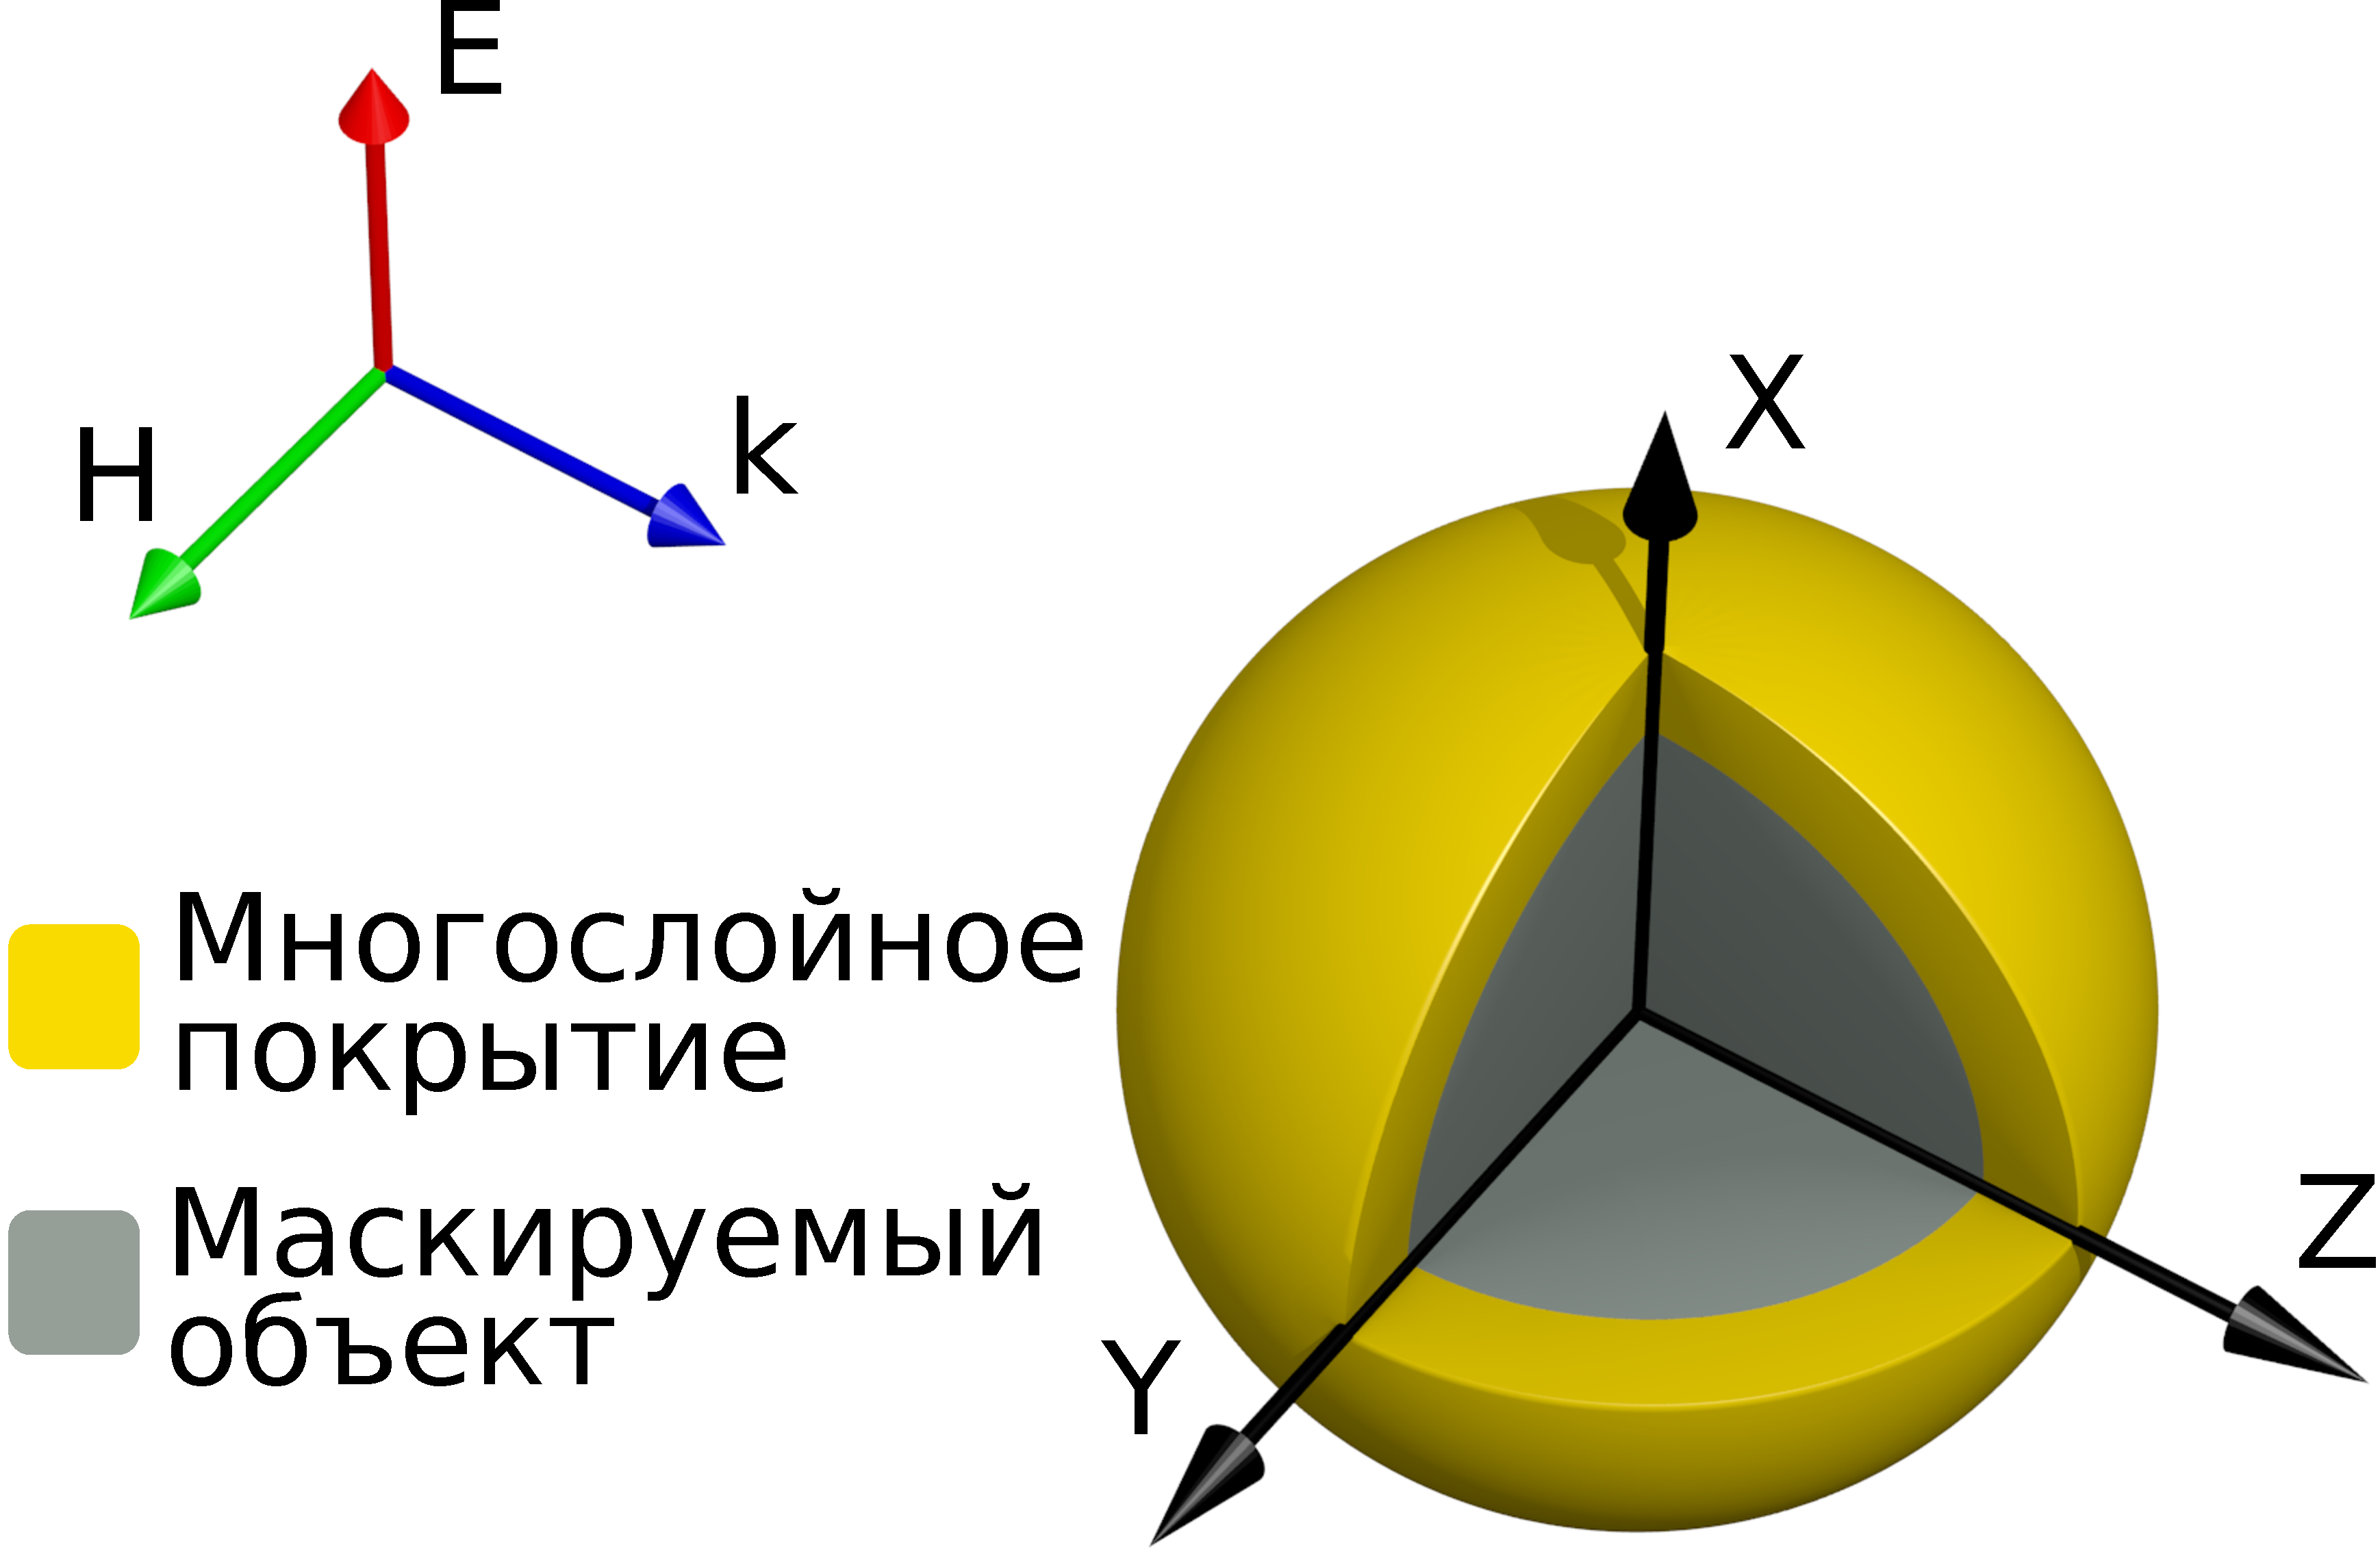
\includegraphics[width=0.57\linewidth]{model-view}}
  \end{minipage}\\
  \vfill
  \begin{minipage}[ht]{0.99\linewidth}
    \centering{а)}
  \end{minipage}\\
  \vfill
  \begin{minipage}[ht]{0.99\linewidth}
    \centering{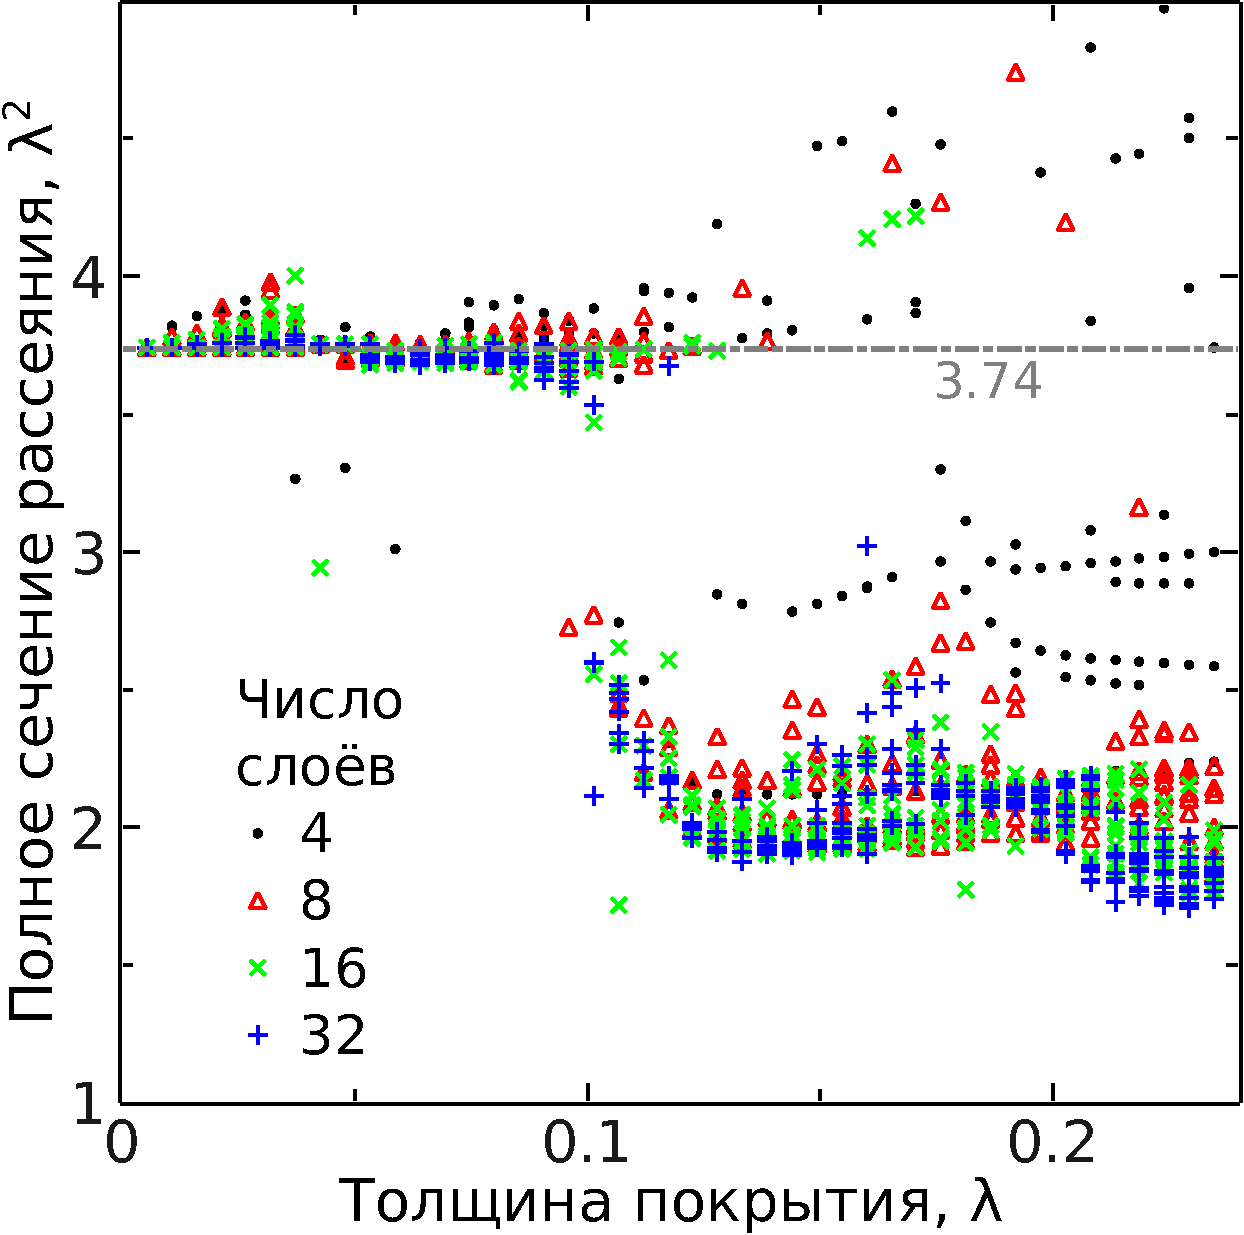
\includegraphics[width=0.57\linewidth]{rcs-overview}}
  \end{minipage}\\
  \vfill
  \begin{minipage}[ht]{0.99\linewidth}
    \centering{б)}
  \end{minipage}
  \vfill

  \caption{(a) Схематическое изображение изучаемой системы:
    маскируемый объект -- сфера из идеального проводящего материала
    внутри многослойного диэлектрического покрытия и падающая
    электромагнитная волна. (б)~Результат работы оптимизатора для
    объекта диаметром $1.5\lambda$.  Каждая отметка на графике
    соответствует одному дизайну покрытия, полученному в результате
    минимизации рассеяния. При толщине покрытия $>0.15\lambda$
    рассеяние можно уменьшить в $\sim 2$ раза.}
  \label{img:scattering}  
\end{figure}

\begin{figure}[p]
  \begin{minipage}[ht]{0.99\linewidth}
    \centering{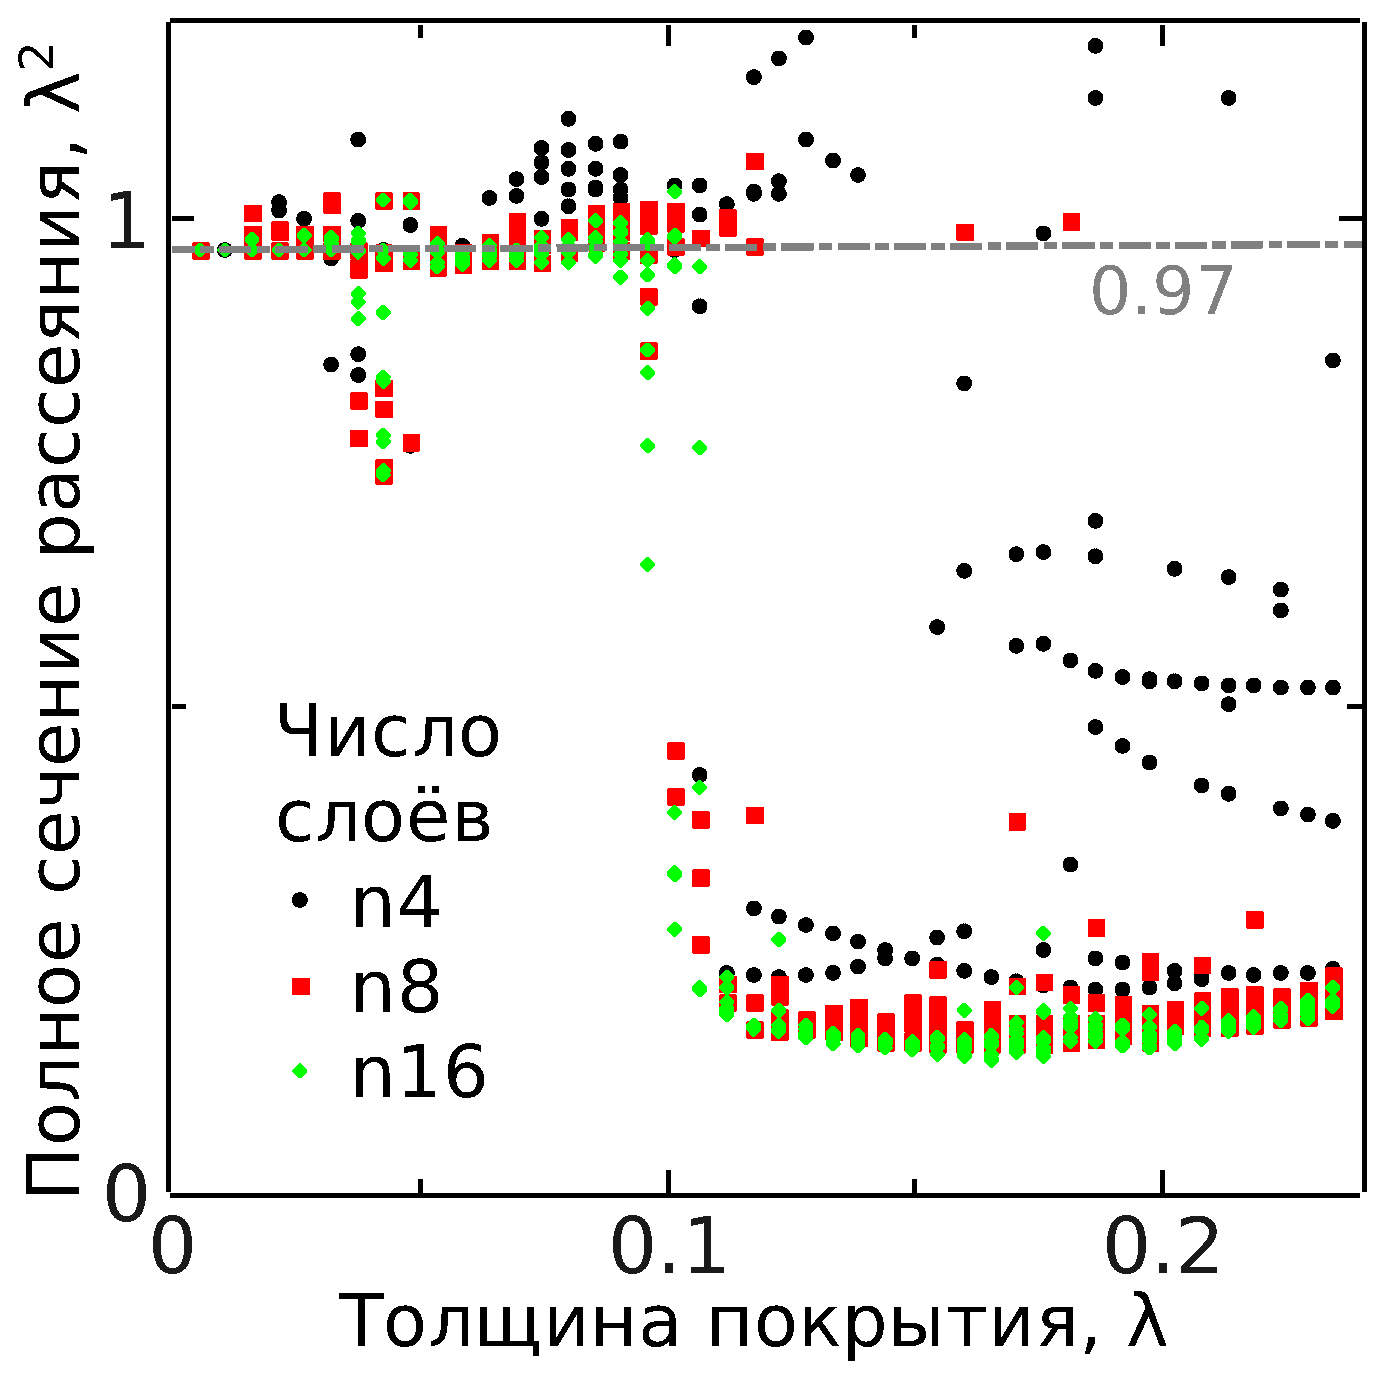
\includegraphics[width=0.57\linewidth]{rcs-overview-r14}}
  \end{minipage}\\
  \begin{minipage}[ht]{0.99\linewidth}
    \centering{а)}
  \end{minipage}\\
  \vfill
  \begin{minipage}[ht]{0.99\linewidth}
    \centering{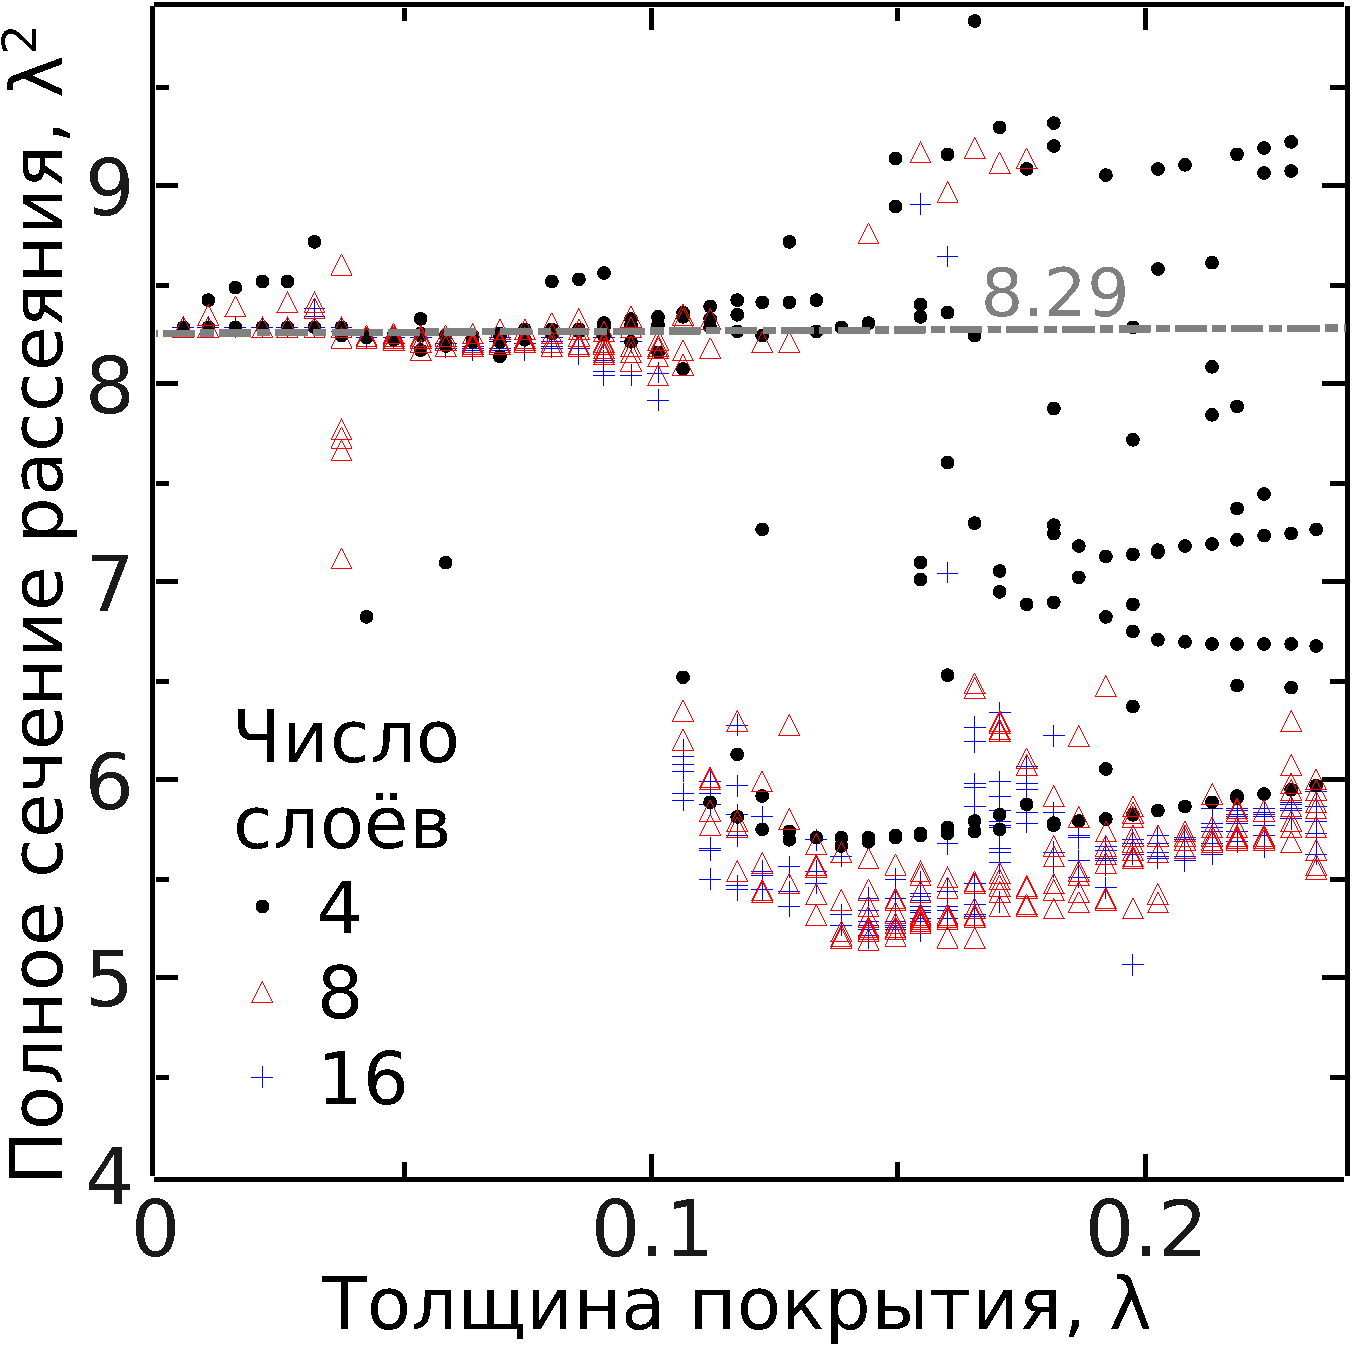
\includegraphics[width=0.57\linewidth]{rcs-overview-r42}}
  \end{minipage}\\
  \begin{minipage}[ht]{0.99\linewidth}
    \centering{б)}
  \end{minipage}
  \vfill
  \caption{Аналогично Рис.~\ref{img:scattering}(б), но для мишени
    (a)~${R_2 = 0.38\lambda}$ и (б)~${R_3 = 1.1\lambda}$.  Типичное
    значение уменьшения TSCS составило приблизительно -85\% и -35\%
    соответственно.  \label{img:rcs-overview-r14-42}}%
\end{figure}


Результат оптимизации в виде зависимости полного сечения рассеяния от
количества слоёв и общей толщины покрытия приводится на
рисунке~\ref{img:scattering}(б) и
рисунках~\ref{img:rcs-overview-r14-42}(а-б). Возможное снижение TSCS
было проверено для разных толщин покрытия в диапазоне от
${W = 0.005\lambda}$ до ${W = 0.235\lambda}$ с шагом $0.005\lambda$ с
помощью серии проходов оптимизации. Были протестированы случаи
разбиения покрытия на 4, 8, 16 (для всех радиусов) и 32 слоя (для
радиуса среднего размера). На рисунках хорошо видно, что существует
некоторое критическое значение для общей толщины покрытия
(${{\rmfamily W}\approx 0.1\lambda}$), до которого дизайнов с
пониженной TSCS относительно непокрытой мишени практически
нет. Большинство дизайнов с пониженной TSCS, обнаруженных
оптимизатором, имеют толщину покрытия выше критической.


Рассмотрим более подробно случай радиуса мишени ${R_1 =
  0.75\lambda}$. Типичное снижение TSCS относительно непокрытой мишени
для толщины выше критической составляет ${\approx -50\%}$ (в два раза
ниже). Непосредственно после превышения критической толщины
превалируют однодолинные
дизайны~(Рис.~\ref{img:designs}(а), на всех графиках
дизайнов в настоящей статье мишень, представленная PEC сферой,
расположена слева, а открытое пространство справа).
\begin{figure}[p]
  \hfill
  \begin{minipage}[ht]{0.44\linewidth}
    \centering{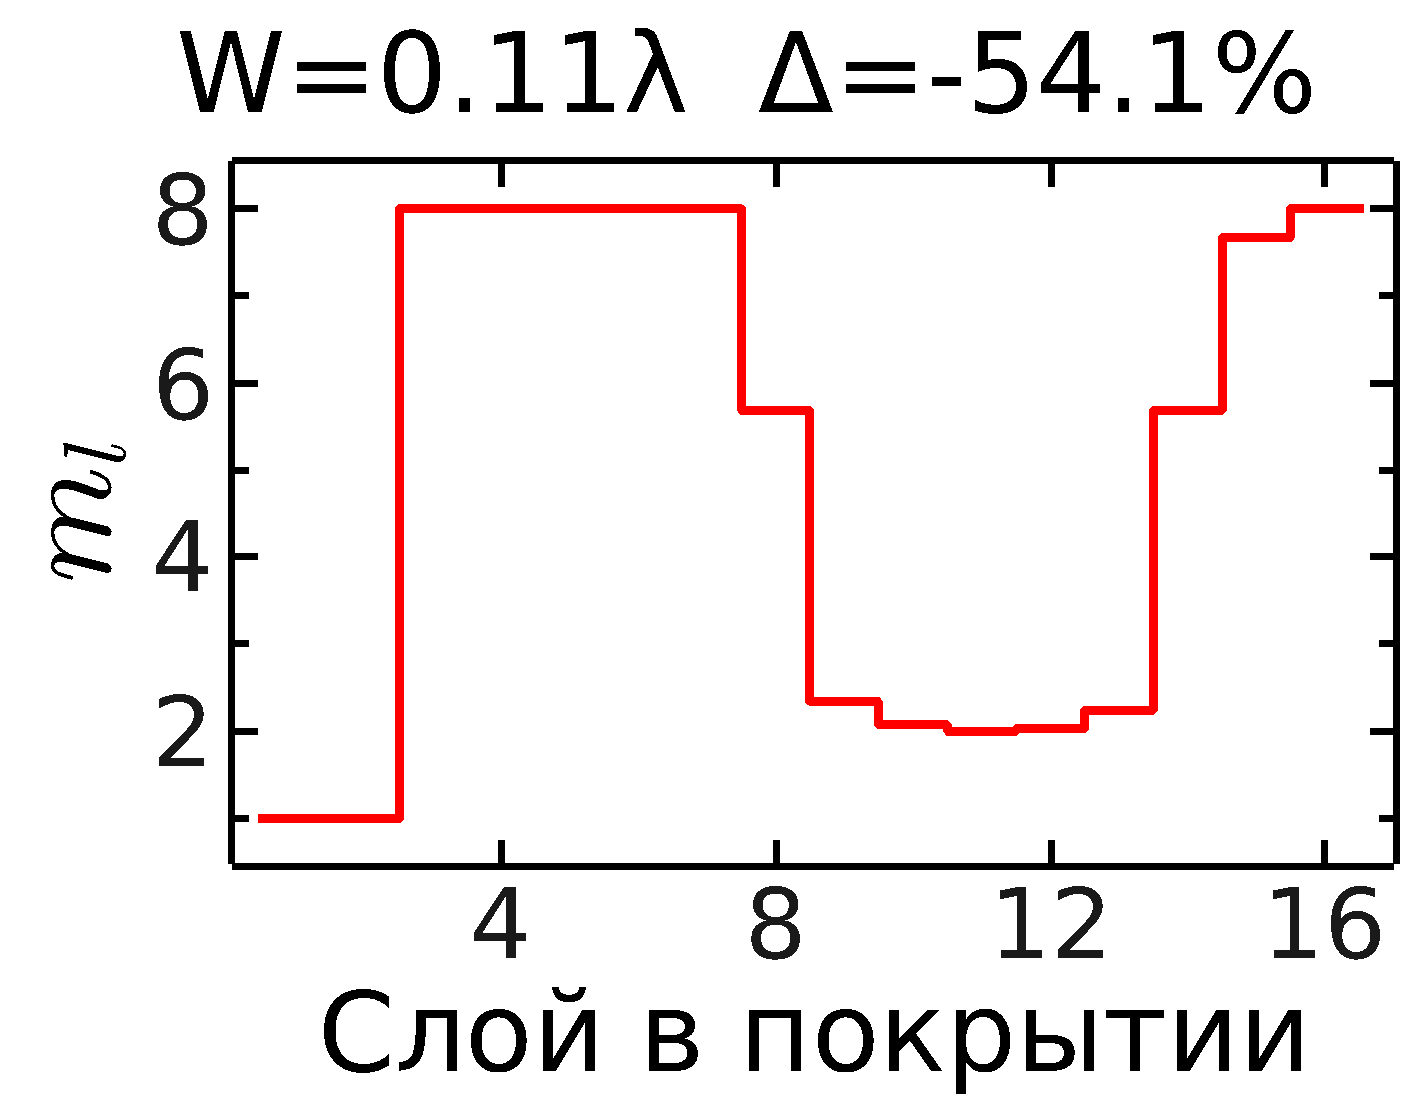
\includegraphics[width=0.95\linewidth]{w04-single-valley-index} \\ а)}
  \end{minipage}
  \hfill
  \begin{minipage}[ht]{0.44\linewidth}
    \centering{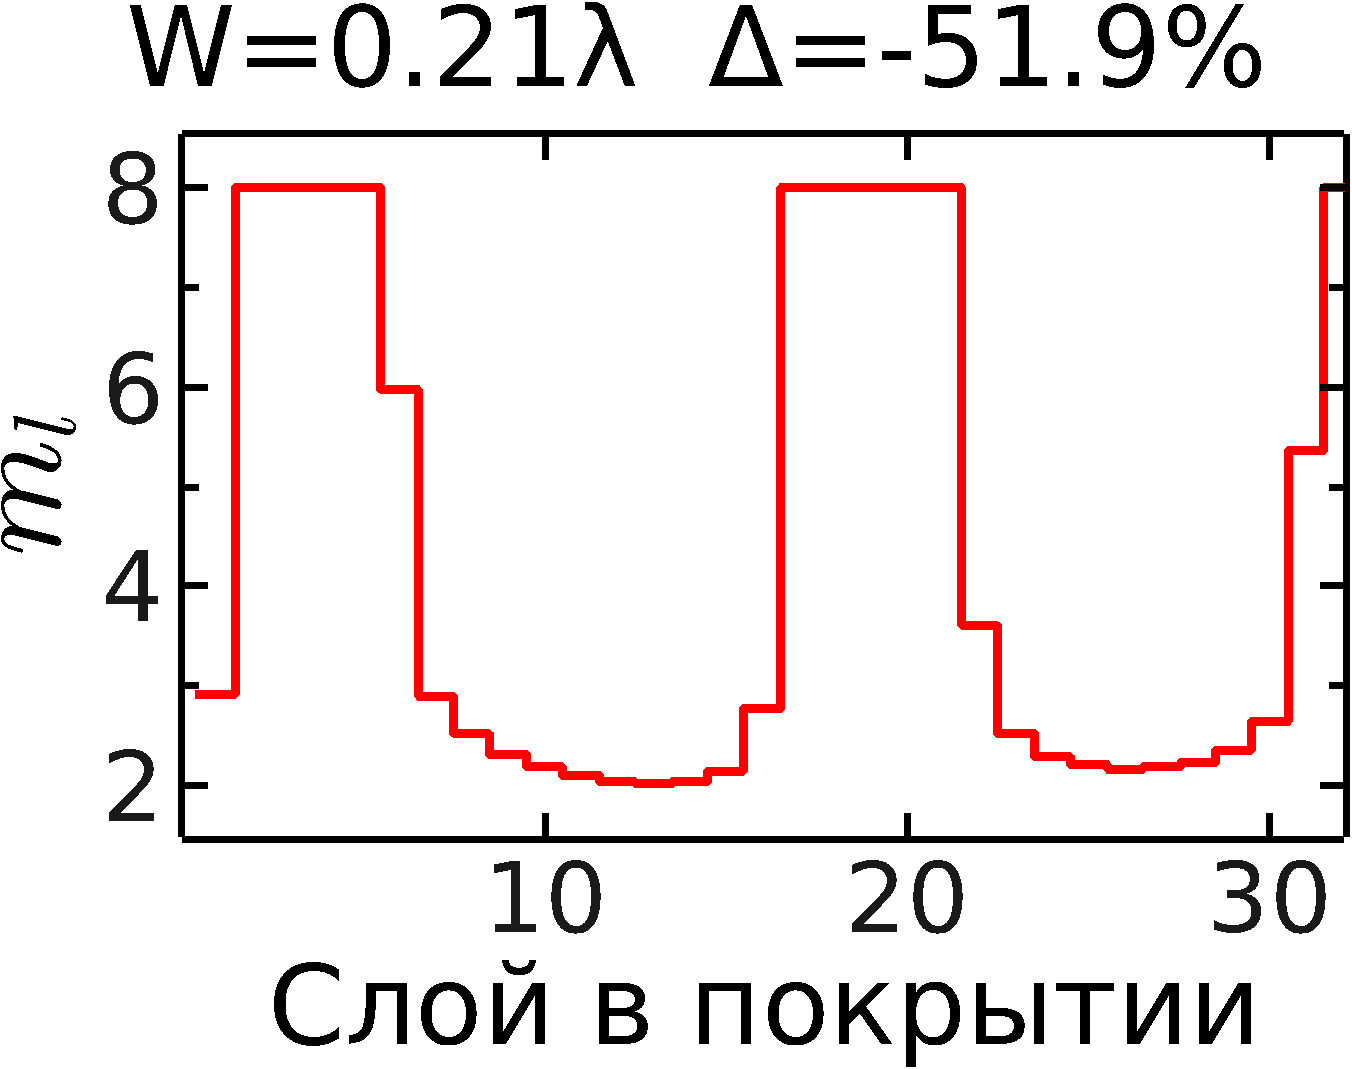
\includegraphics[width=0.95\linewidth]{w08-double-valley-index} \\ б)}
  \end{minipage}
  % \begin{minipage}[ht]{0.32\linewidth}
  %   \centering{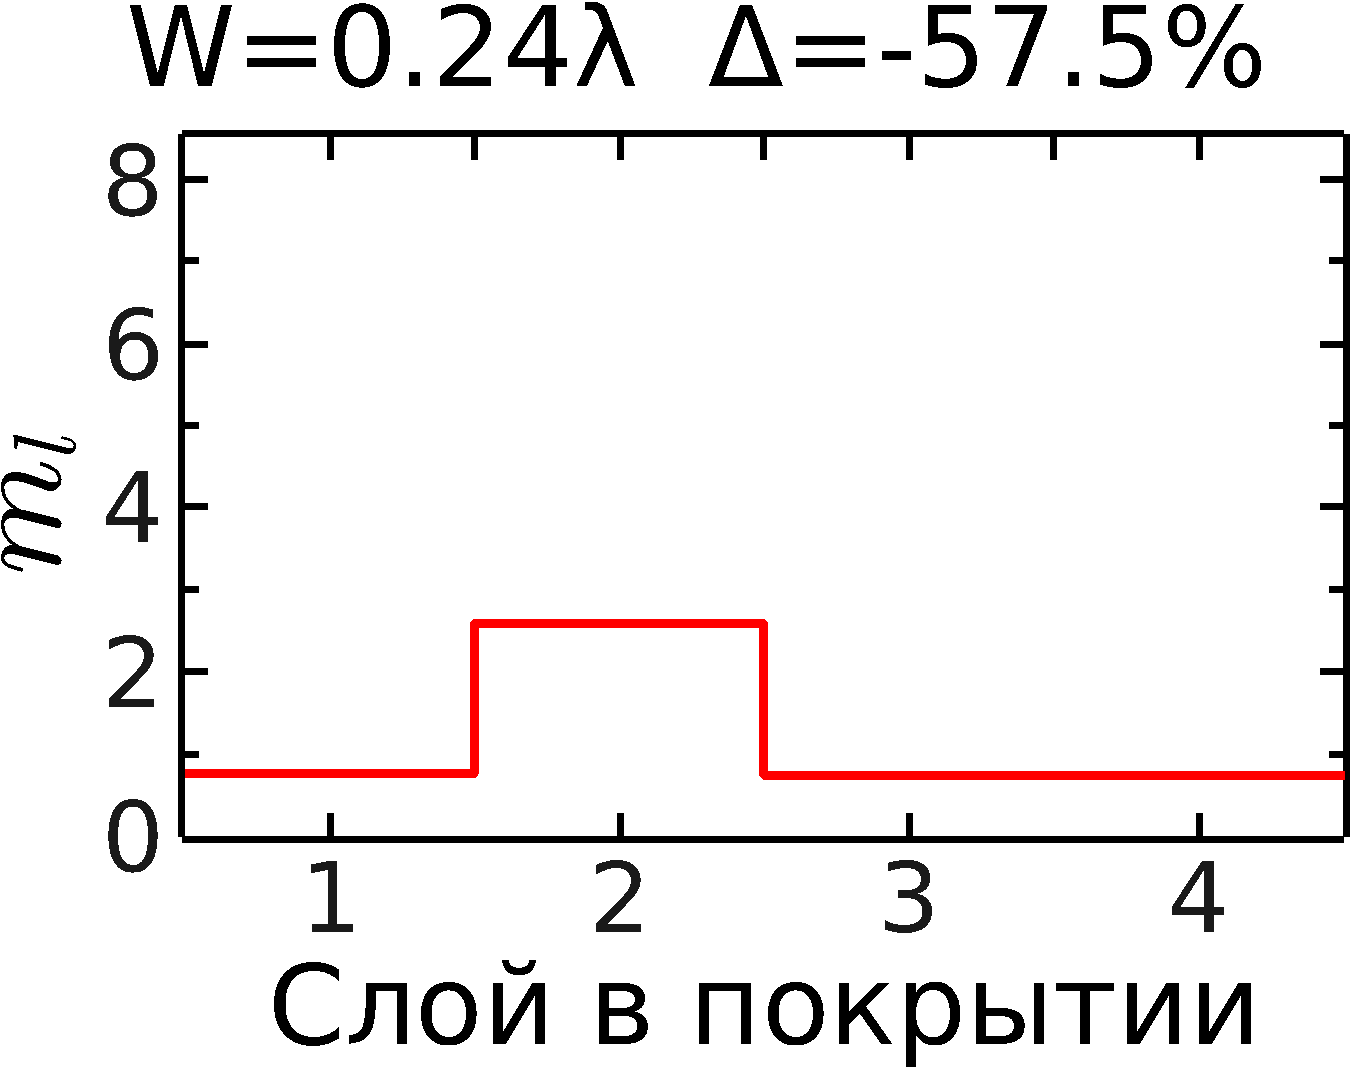
\includegraphics[width=0.95\linewidth]{index07-TO} \\ в)}
  % \end{minipage}
  \caption{Типичные дизайны, обеспечивающие наилучшую маскировку при
    толщине покрытия, равной (a)~$0.11\lambda$ и
    (б)~$0.21\lambda$. Максимальное значение показателя преломления
    было ограничено $n_{\mathrm{max}}=8$, а минимальное значение было
    равно $n_{\mathrm{min}}=1$ }
  \label{img:designs}  
\end{figure}
\begin{figure}[p]
  \begin{minipage}[ht]{0.495\linewidth}
    \centering{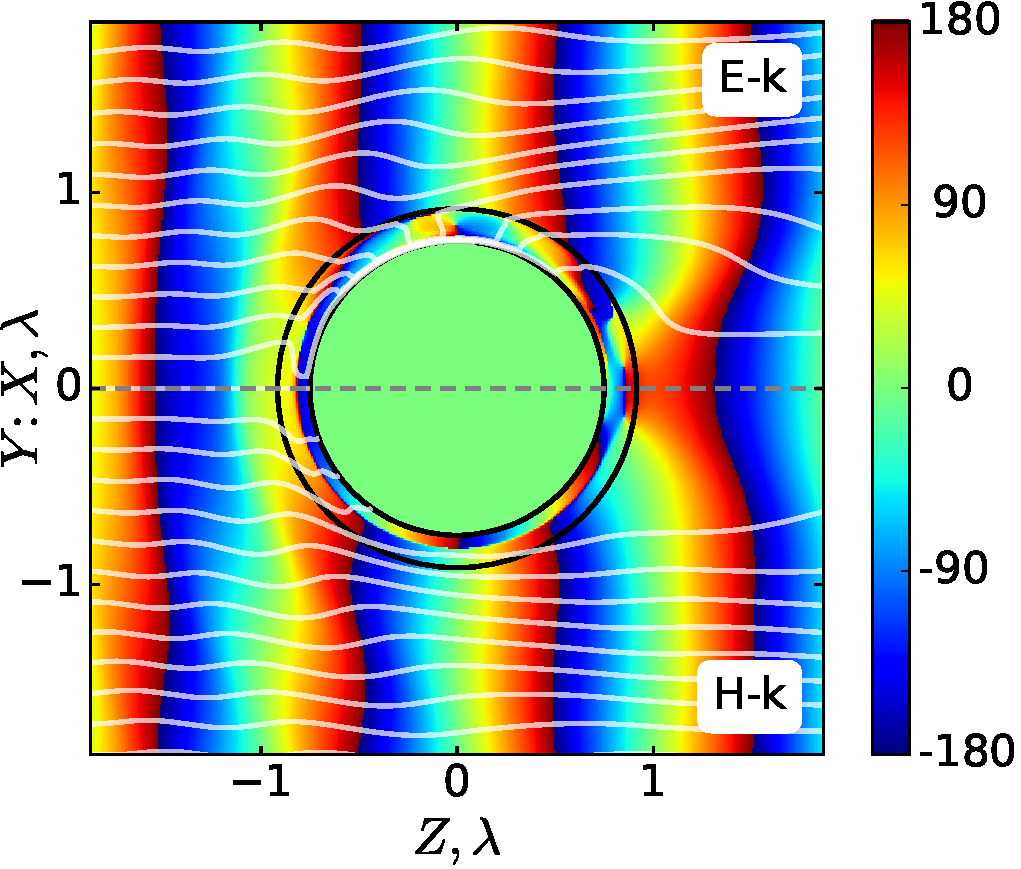
\includegraphics[width=0.98\linewidth]{PEC-index-sv-R3-XYZ-angleEx} \\ а)}
  \end{minipage}
  \hfill
  \begin{minipage}[ht]{0.495\linewidth}
    \centering{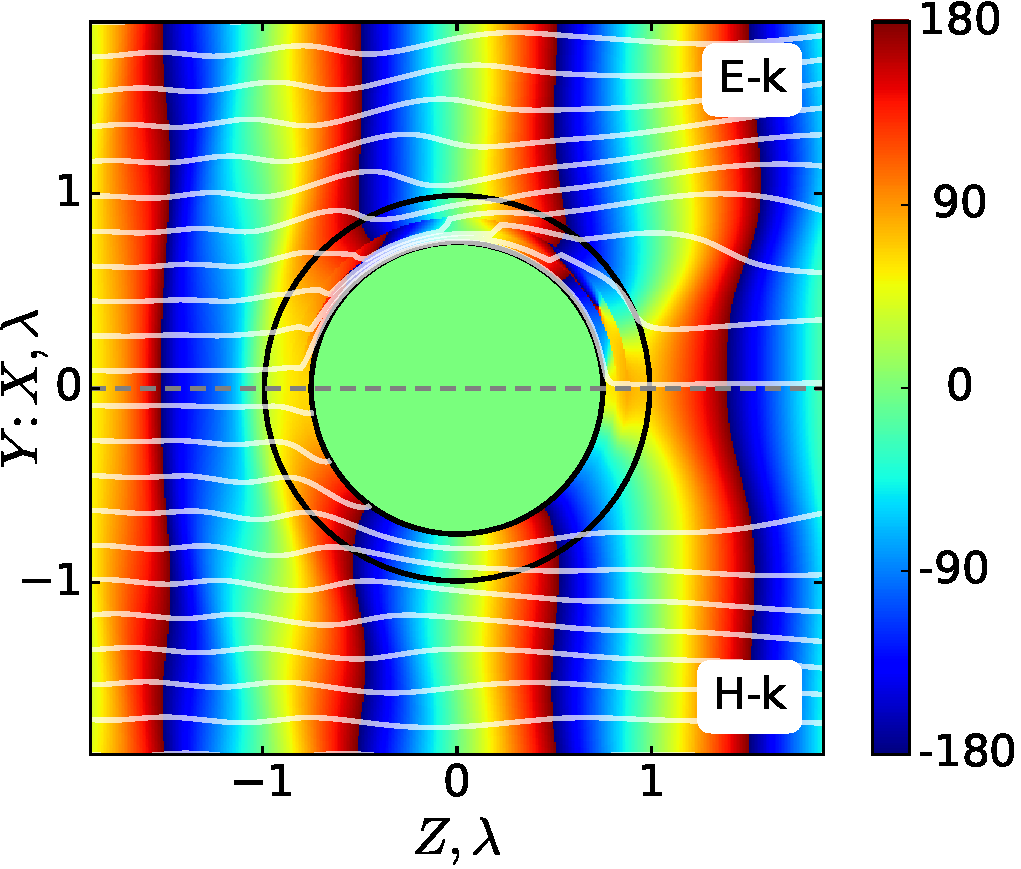
\includegraphics[width=0.98\linewidth]{PEC-index-in-glass-R1-XYZ-angleEx} \\ б)}
  \end{minipage}
  \caption{Изображение фазы электрического поля в случае маскировки
    объекта покрытием из изотропных (а) диэлектриков
    (см.~рисунок~\ref{img:designs}(а)) и (б) материалов с
    ${\varepsilon <1}$ (см.~рисунок~\ref{img:designs}(в)). Изображения
    построены в виде эпюра из плоскости поляризации падающей волны
    (верхняя половина) и перпендикулярной плоскости (нижняя
    половина). Чёрные окружности маркируют границы маскирующего
    покрытия. Белым обозначены линии потока энергии, волна
    распространяется в плоскости рисунка слева направо.}
  \label{img:field-phase}  
\end{figure}
Такие дизайны, как правило, начинаются с воздушного промежутка между
покрытием и мишенью из PEC, затем следует быстрое увеличение
показателя преломления до максимально допустимого. После нескольких
слоёв с высоким значением величина показателя преломления постепенно
идёт вниз и снова вверх, образуя долину с низким значением внутри двух
стенок с высоким значением. Минимальное значение показателя
преломления в долине обычно оказывается около двух. За второй стенкой
долины величина показателя преломления резко падает с высокого значения до
уровня воздуха.

Наряду с ростом толщины от ${\approx 0.62}$~см до ${\approx 0.78}$~см
происходит переход ~(Рис.~\ref{fig:transition}) от
однодолинного~(Рис.~\ref{fig:single-valley-index-design}) к
двухдолинному~(Рис.~\ref{fig:CST-index-design}) дизайну, где оба
дизайна сосуществуют при одной и той же толщине.

\begin{figure}[p]
  \begin{minipage}[h]{0.45\textwidth}
    \centering{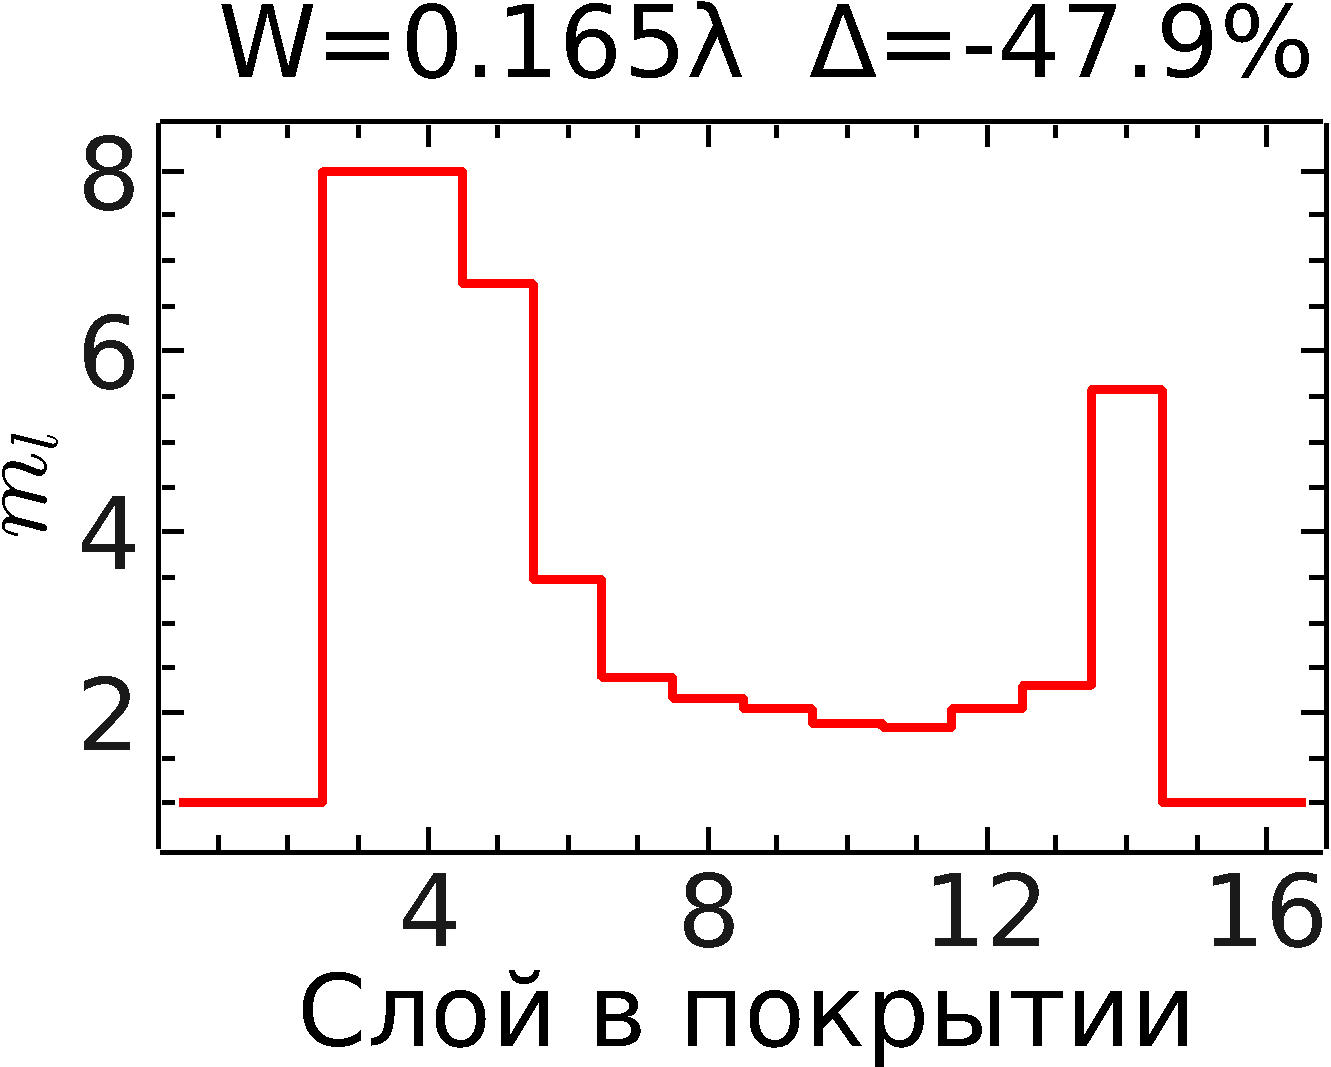
\includegraphics[width=0.99\textwidth]{w062-s-diff-479}\\а)}
  \end{minipage}
  \begin{minipage}[h]{0.45\textwidth}
    \centering{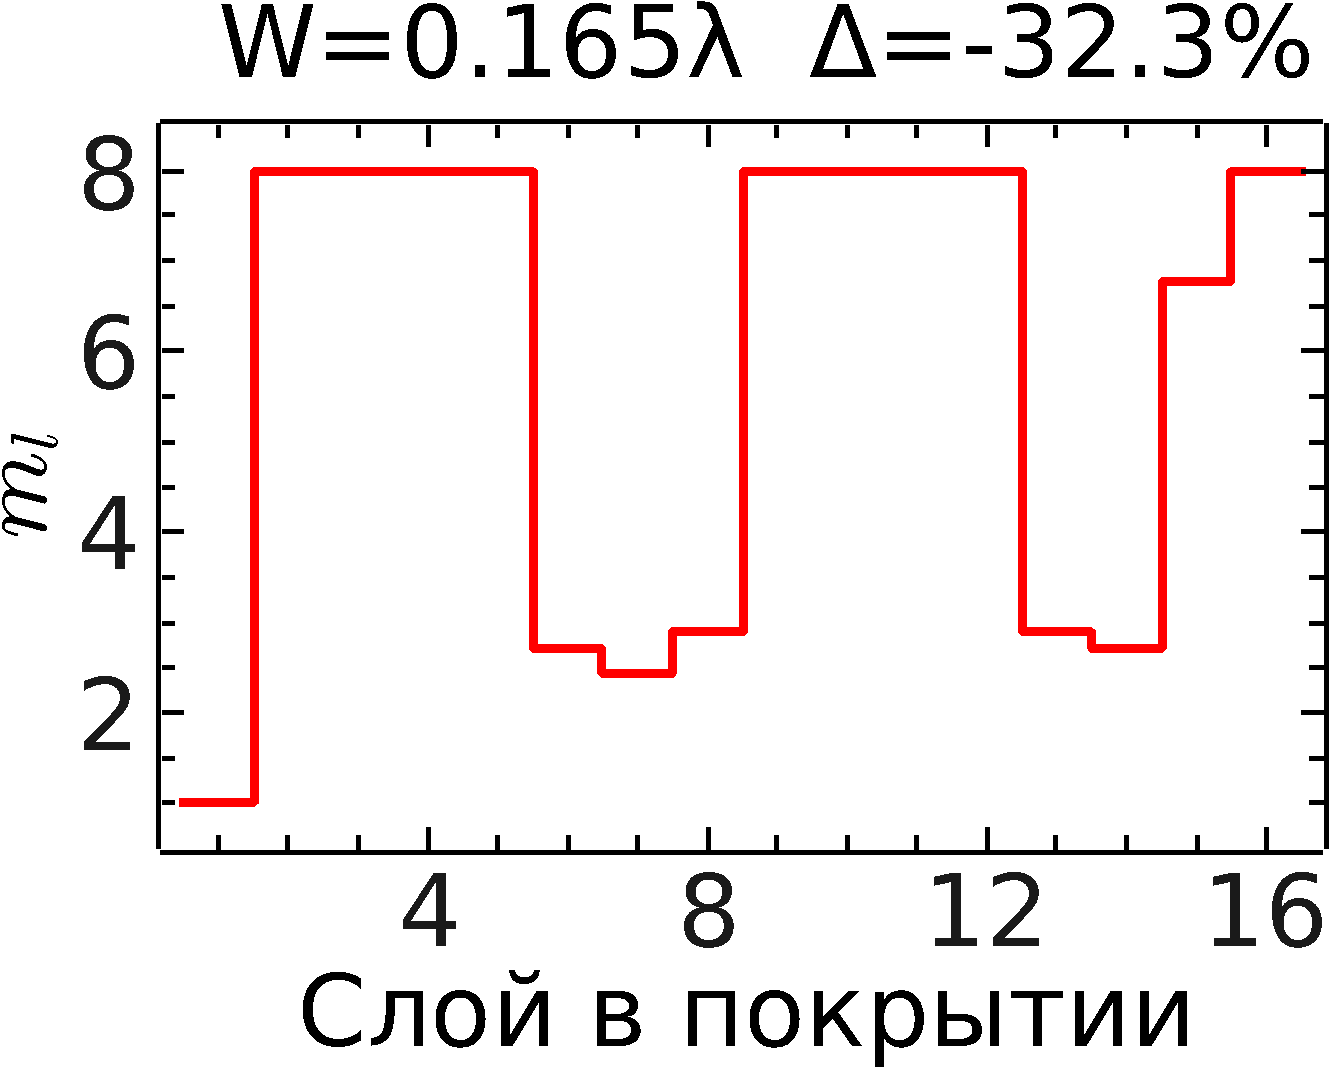
\includegraphics[width=0.99\textwidth]{w062-t-diff-323}\\б)}
  \end{minipage}\\
  \vspace{12pt}\\
  \begin{minipage}[h]{0.45\textwidth}
    \centering{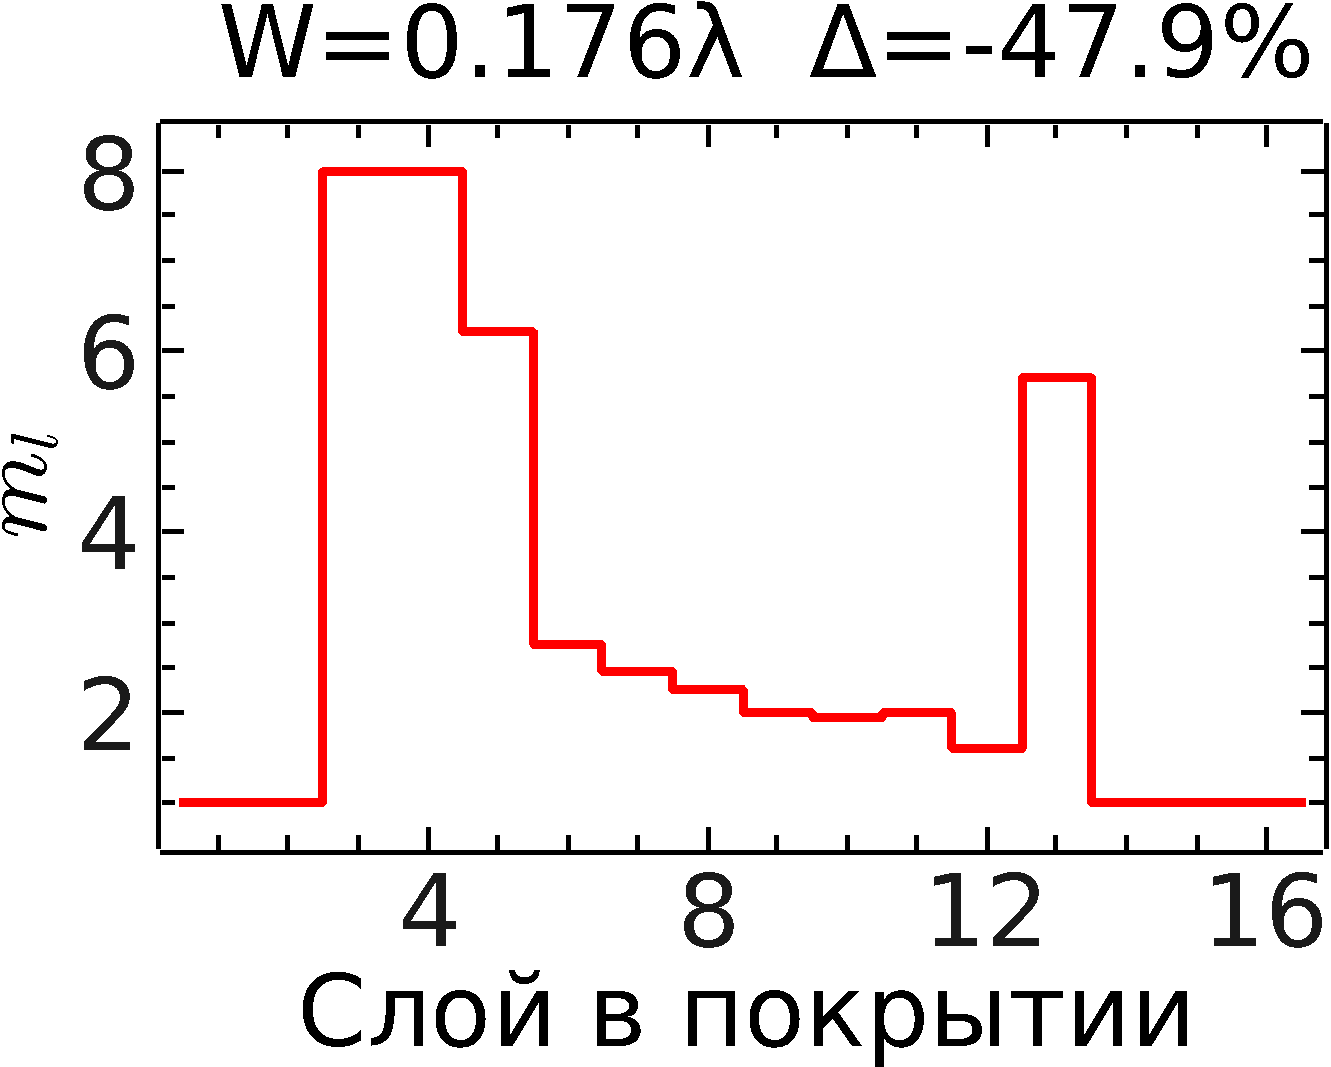
\includegraphics[width=0.99\textwidth]{w066-s-diff-479}\\в)}
  \end{minipage}
  \begin{minipage}[h]{0.45\textwidth}
    \centering{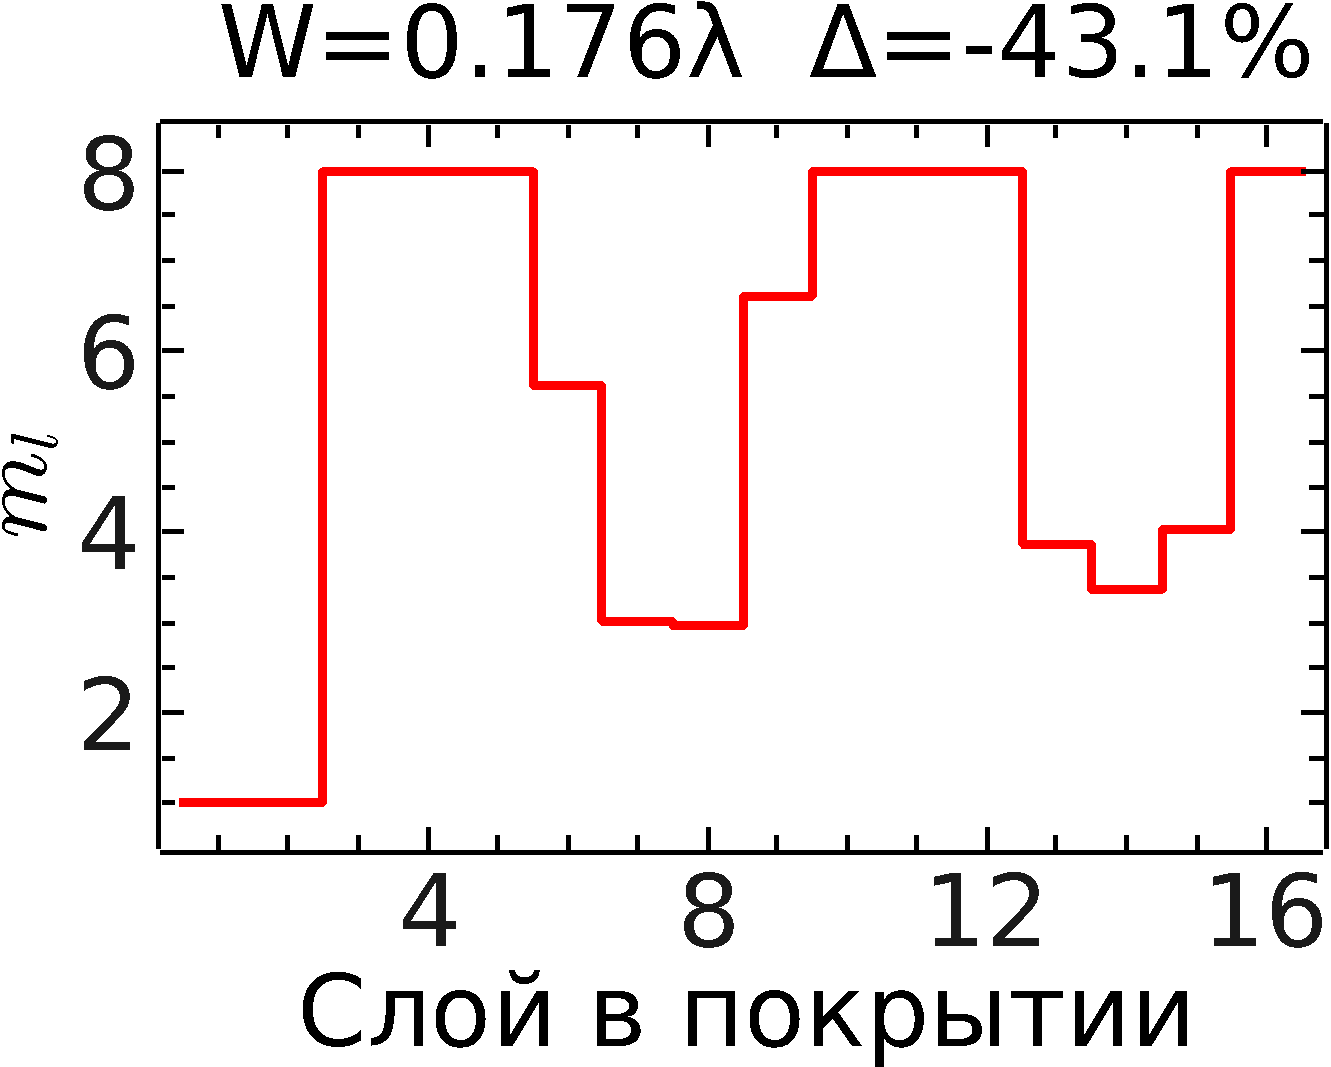
\includegraphics[width=0.99\textwidth]{w066-t-diff-431}\\г)}
  \end{minipage}\\
  \vspace{12pt}\\
  % \begin{minipage}[h]{0.45\textwidth}
  %   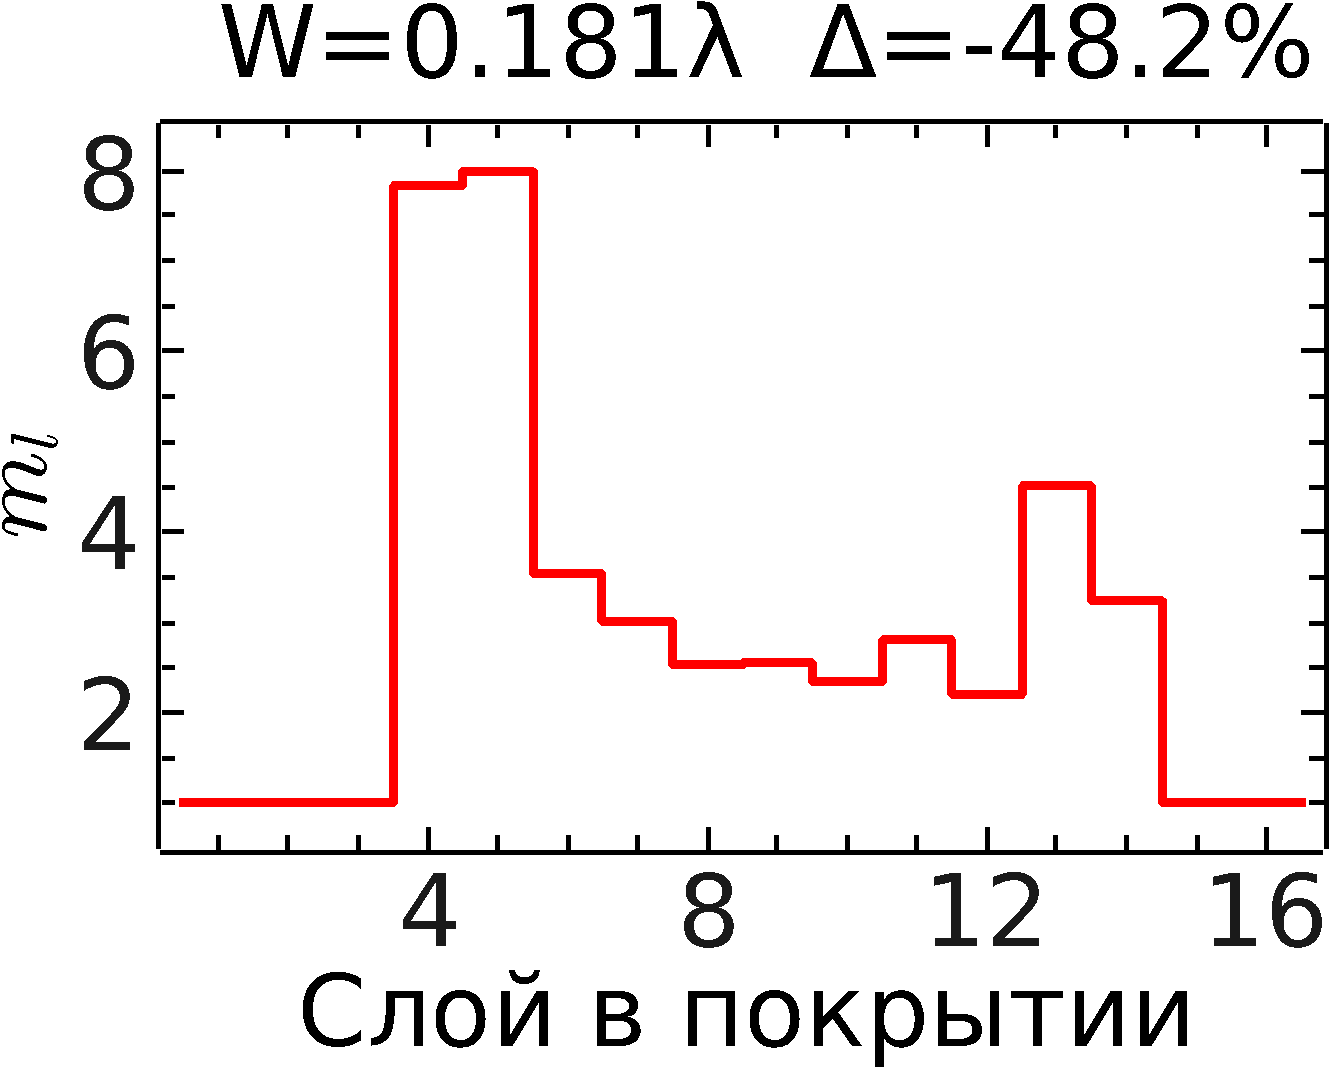
\includegraphics[width=0.99\textwidth]{w068-s-diff-482}
  % \end{minipage}
  % \begin{minipage}[h]{0.45\textwidth}
  %   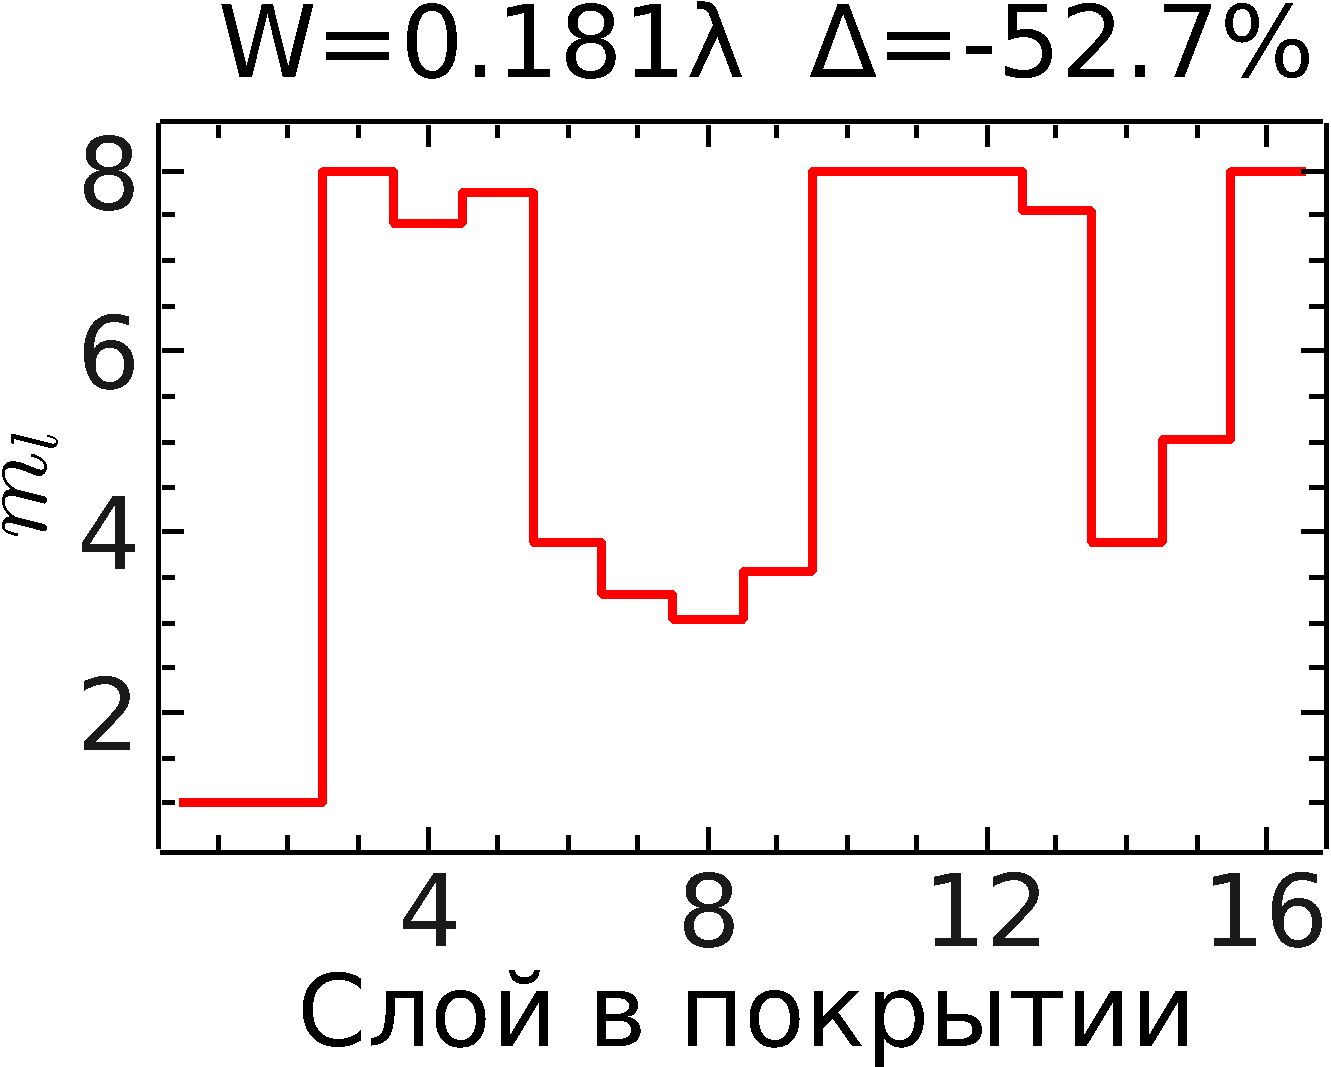
\includegraphics[width=0.99\textwidth]{w068-t-diff-527}
  % \end{minipage}\\
  % \vspace{12pt}\\
  \begin{minipage}[h]{0.45\textwidth}
    \centering{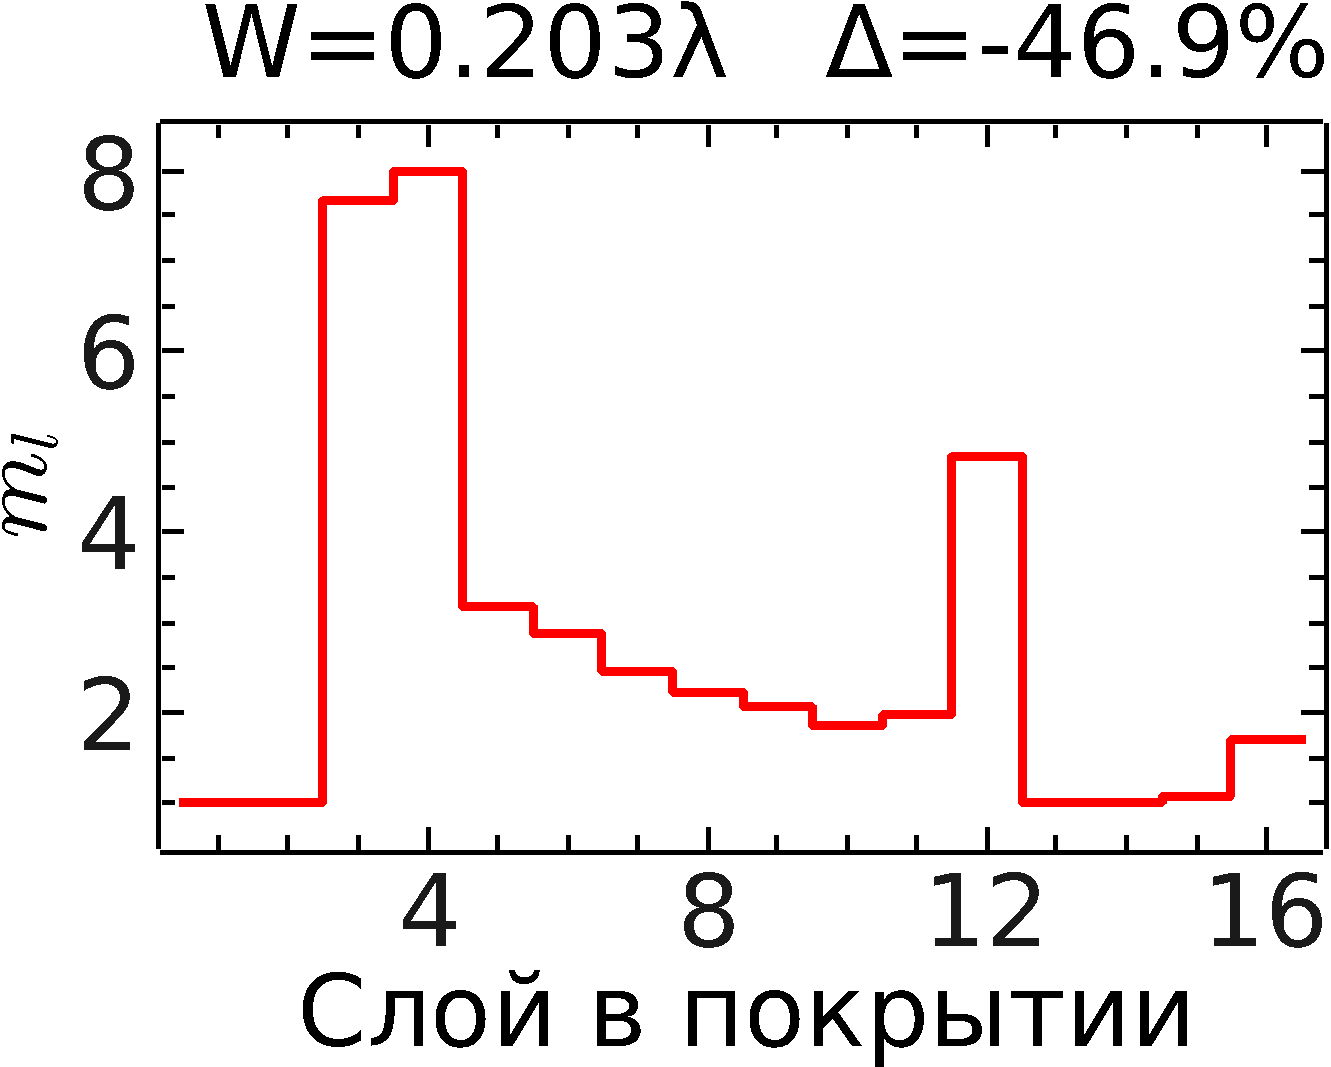
\includegraphics[width=0.99\textwidth]{w076-s-diff-469}\\д)}
  \end{minipage}
  \begin{minipage}[h]{0.45\textwidth}
    \centering{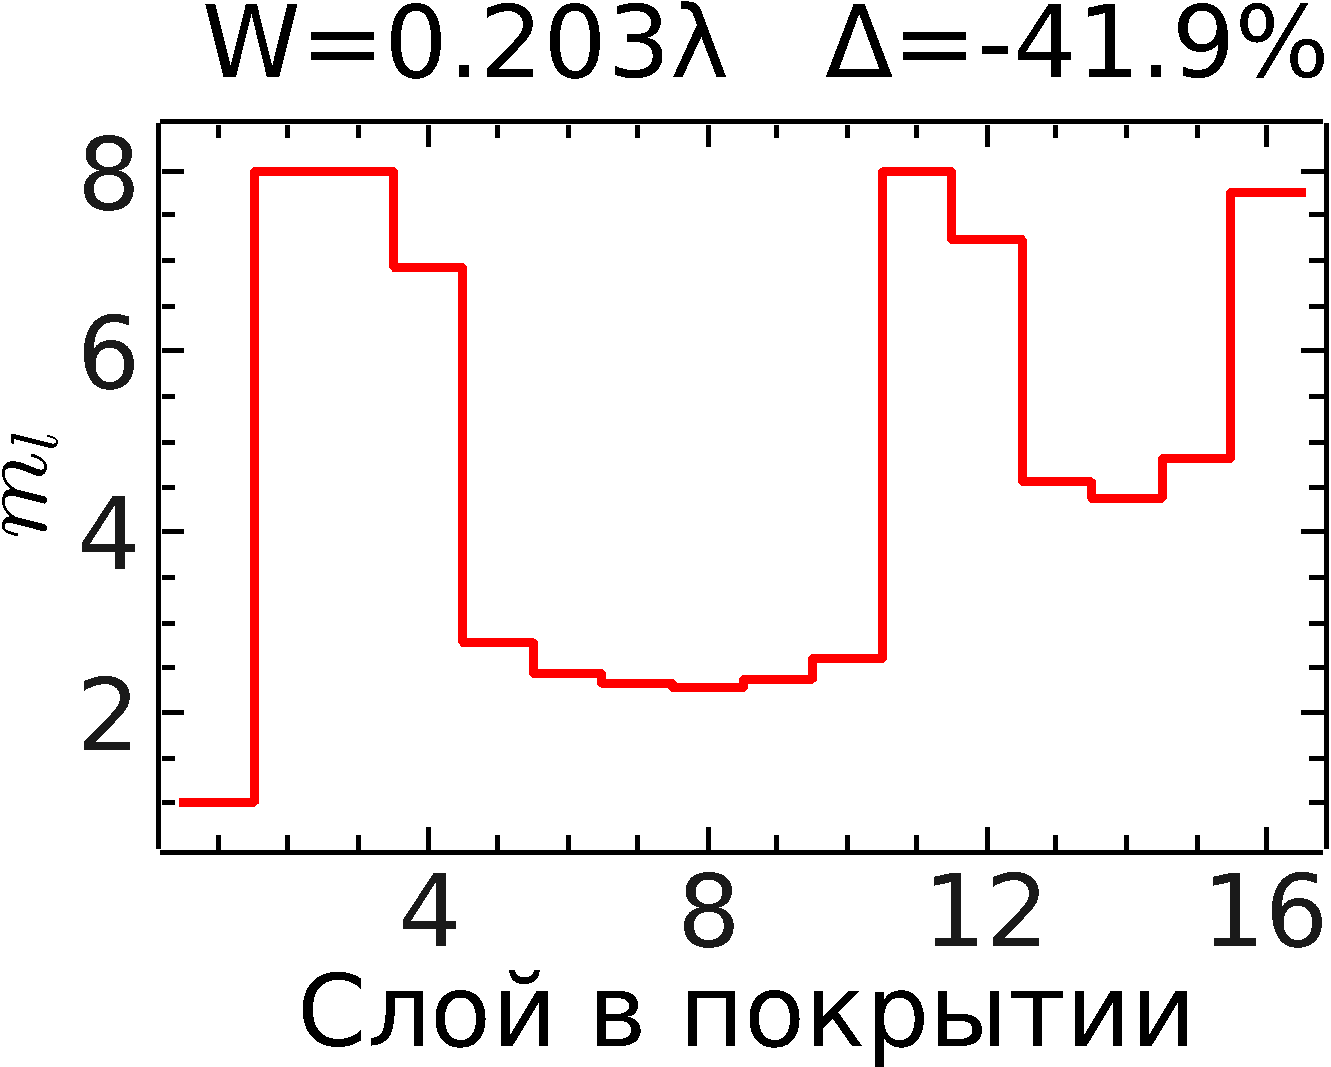
\includegraphics[width=0.99\textwidth]{w076-t-diff-419}\\е)}
  \end{minipage}%
  \caption{Переход от однодолинного к двухдолинному дизайну. Каждой
    паре (а-б), (в-г) и (д-е) соответсвует одинаковая толщина
    покрытия. Каждый профиль показателя преломления был получен
    независимо, в отдельном проходе оптимизации.
    \label{fig:transition}}%
\end{figure}
Для толщины покрытия более ${\approx 0.68}$~см большинство дизайнов
имеет двухдолинную конфигурацию, немногие остальные не в полной мере
соответствуют однодолинной модели из-за наличия в покрытии внутреннего или
внешнего слоя с относительно высоким значением показателя
преломления. Для толщины выше ${\approx 0.78}$~м однодолинных дизайнов
обнаружено не было.

Во время перехода однодолинный дизайн представляется довольно
стабильным, поскольку он достиг наилучшего состояния. Двухдолинный
дизайн, видимо, ограничен допустимой толщиной покрытия. С увеличением
толщины покрытия ширина долин также увеличивается. Ширина внутренней
долины (которая ближе к PEC мишени) растёт быстрее. Это может быть
связано со следующим фактом: электромагнитное поле в покрытии в
основном сосредоточено во внутренних слоях
(Рис.~\ref{fig:CST-Ex}). Таким образом, дизайн внутренних слоёв
оказывает более сильное воздействие на итоговую TSCS по сравнению с
наружными слоями; следовательно, внутренние слои имеют приоритет при
оптимизации.

Существенного дополнительного снижения TSCS после перехода
не наблюдается. Мы полагаем, что также возможны многодолинные дизайны;
однако мы не смогли получить их из-за ограничений по времени и по
вычислительным мощностям. Была проведена быстрая попытка оптимизации
для толщины покрытия 2.4~см, для которой оптимизатор смог найти некий
дизайн~(Рис.~\ref{fig:thick}) с 54.3\% падением TSCS.
\begin{figure}
  \centering{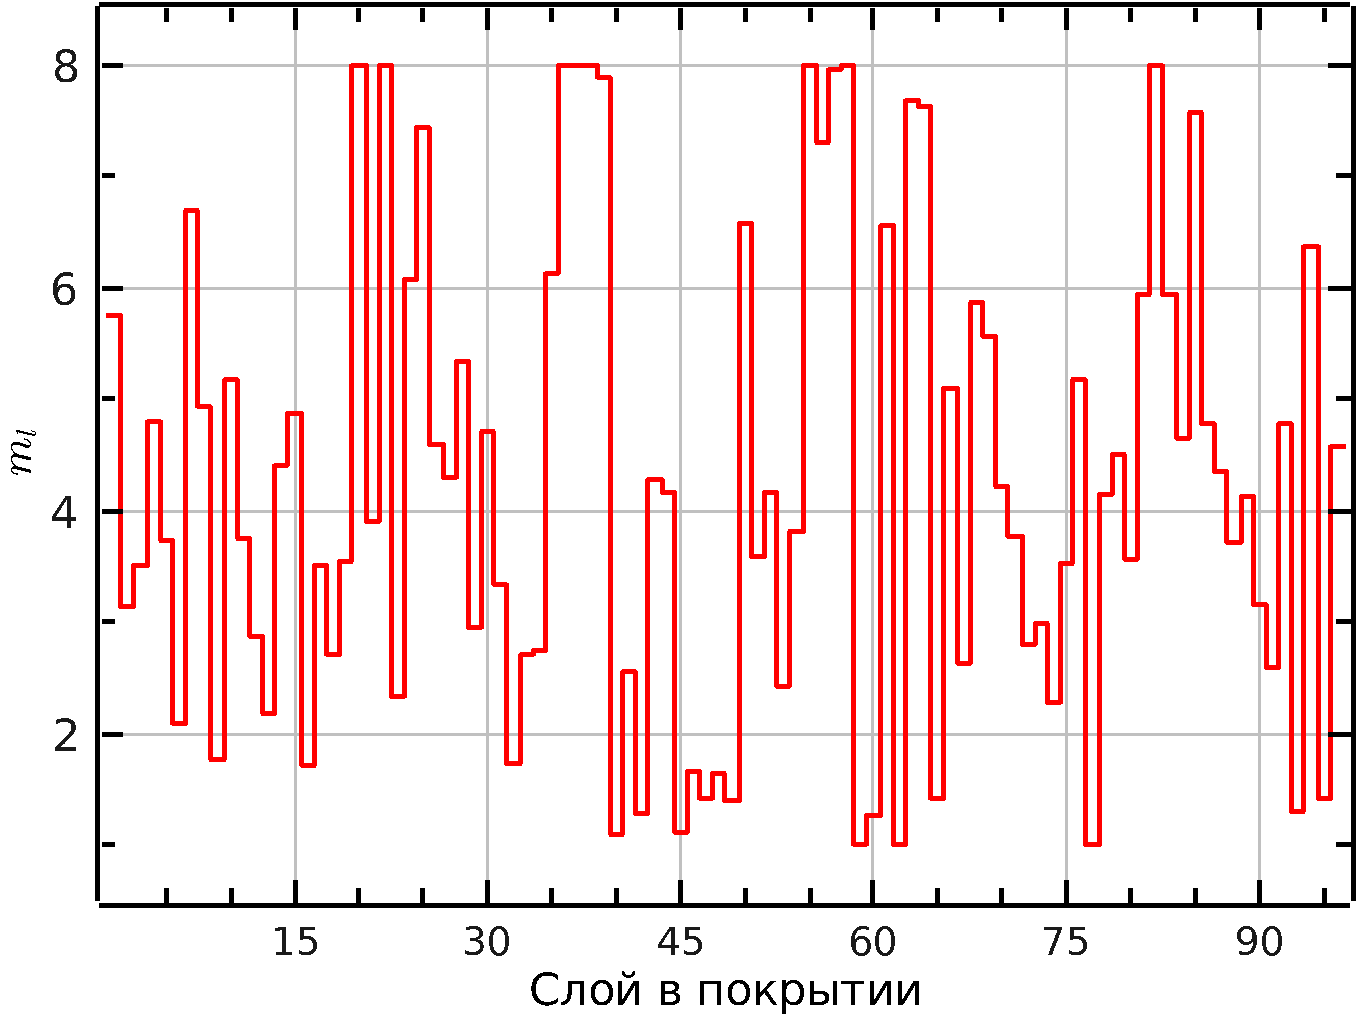
\includegraphics[width=0.87\textwidth]{w24-chaotic-index}}%
  \caption{Хаотический дизайн для толщины покрытия $W=2.4$~cm
    $\Delta =-54.3$\% после 10~000 поколений.
    \label{fig:thick}}%
\end{figure}
К сожалению, он выглядит довольно хаотично и не поддаётся простой
классификации.

%БЛОК 2

Необходимо отметить, что <<дёрганое>> поведение профиля показателя
преломления, хорошо видное в случае хаотического дизайна, может быть
частично обнаружено в случаях однодолинного и двухдолинных дизайнов,
описанных выше.  Это можно объяснить следующим образом: толщина
отдельного слоя внутри покрытий в десятки раз меньше длины волны (слои
являются субволновыми).  Таким образом, если поменять местами два
соседних слоя, то эффективное значение показателя преломления
поменяется слабо, и будет наблюдаться сопоставимая величина падения
TSCS.  В случае, если разница в величине показателя преломления между
этими слоями оказывается достаточно большой, то будет наблюдаться
<<дёрганое>> поведения профиля показателя преломления.  Подобное
поведение тонких многослойных покрытий представляет
существенную сложность для любого алгоритма оптимизации, так как очень
похожие друг на друга с физической точки зрения системы оказываются
сильно удалены друг от друга в многомерном пространстве входных
параметров.  Иначе говоря, у целевой функции, используемой в качестве
критерия оптимизации, наблюдаются многочисленные локальные
минимумы.  Этот факт при использовании стохастического оптимизатора
приводит к тому, что конечный результат каждого прохода может
оказаться немного другим.  По этой причине для каждого набора входных
параметров выполнялась серия проходов оптимизации, а это, в свою
очередь, обусловило наличие нескольких отметок одного типа
(одно и то же количество слоёв в покрытии) для каждой исследованной
толщины покрытия~(Рис.~\ref{fig:rcs-overview},%
~\ref{fig:rcs-overview-r14},~\ref{fig:rcs-overview-r42}), отметки с
большим значением величины TSCS обычно обладают более <<дёрганым>>
профилем показателя преломления.  В целом, несмотря на указанные
сложности, адаптивный метод дифференциальной эволюции воспроизводимо
находит дизайны  с уменьшенным рассеянием в выбранном диапазоне толщин
и числа слоёв в разбиении.

Как следует из Рис.~\ref{fig:rcs-overview}, разбиения покрытия на
четыре слоя оказывается недостаточным для достижения оптимальных
значений TSCS.  Большинство дизайнов, обладающих TSCS более 35~см$^2$ и
толщиной покрытия, превышающей критическую, используют разбиение на 4
слоя.  При этом разбиения на 8 слоёв оказывается достаточным для того,
чтобы получить результаты, сравнимые со случаями 16 и 32 слоёв
(особенно для диапазона толщин покрытия, соответствующих однодолинному
дизайну).  Тем не менее, у разбиения на 32 слоя есть небольшое
преимущество в случае большой толщины покрытия (${> 0.8}$~см).

Как было указано ранее, обнаружено небольшое число дизайнов с
маскирующим эффектом в случае толщины покрытия значительно меньше
критической.  Чтобы изучить такие дизайны мы провели дополнительную серию
оптимизаций (треугольники без заполнения на Рис.~\ref{fig:rcs-overview-thin}).
\begin{figure}
  \centering{
    % Use pdfcrop to remove white margins
    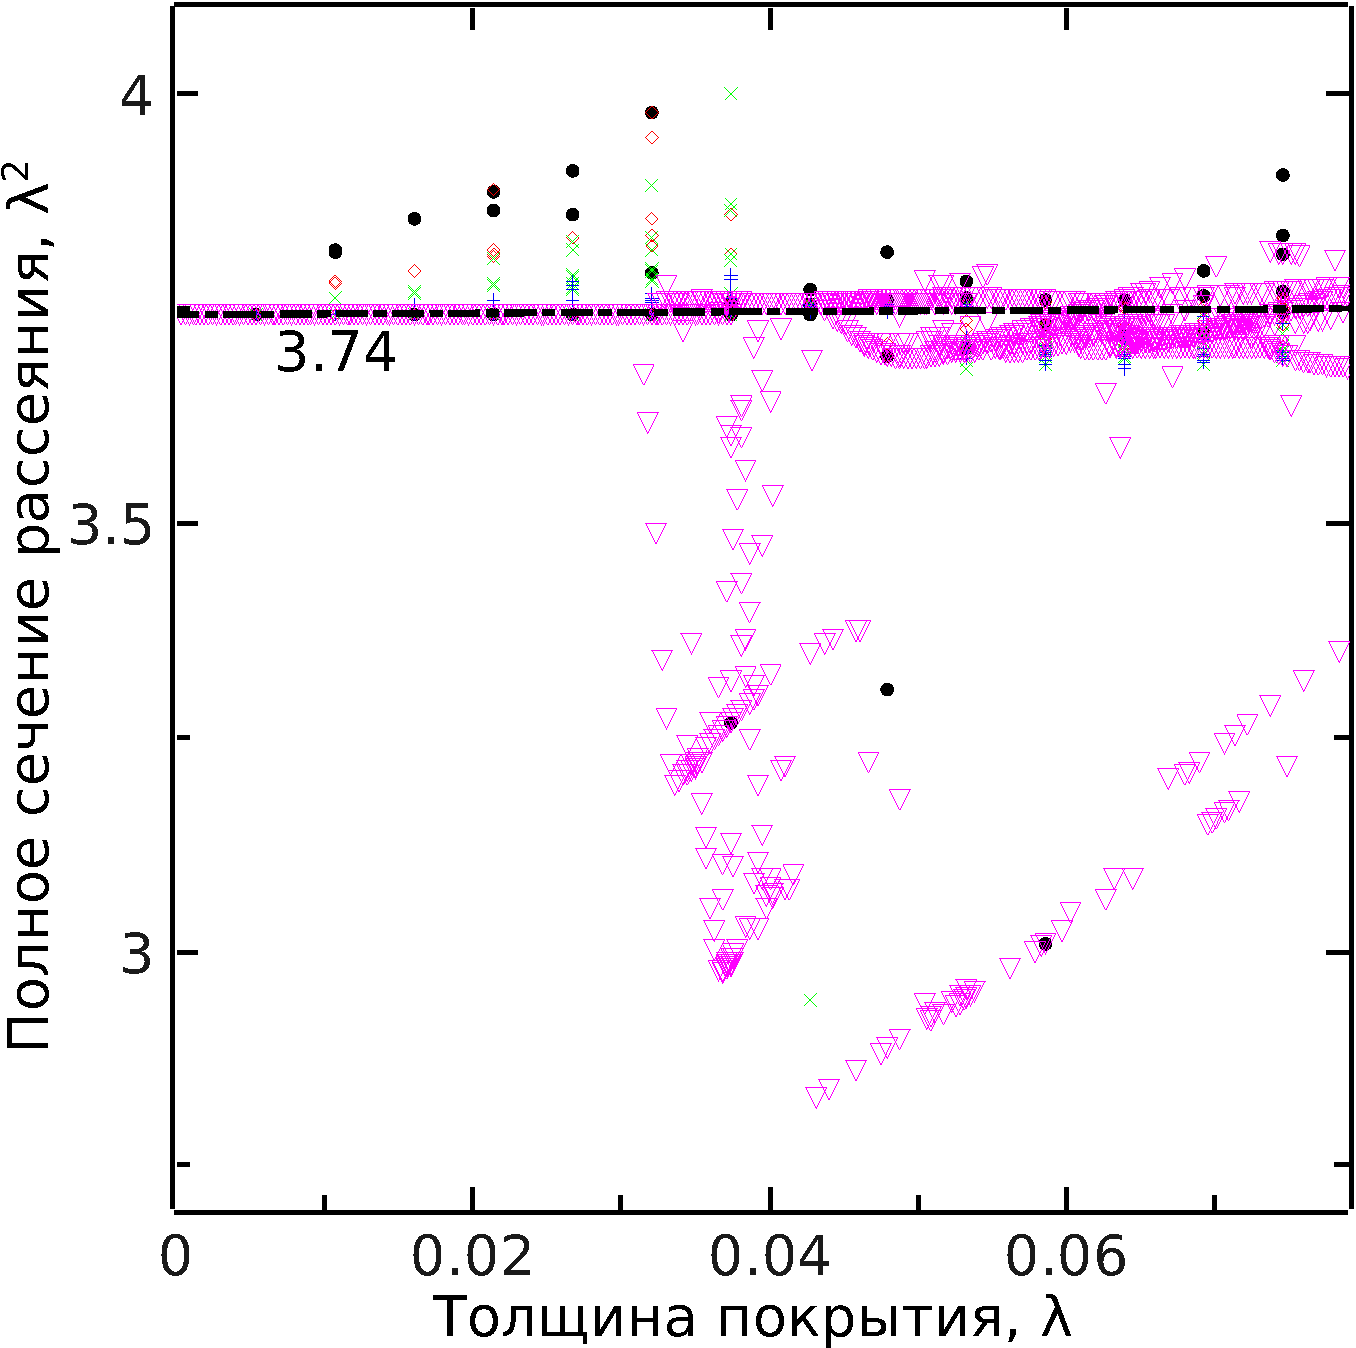
\includegraphics[width=0.47\textwidth]{rcs-overview-thin}%
      \caption{Увеличенная часть Рис.~\ref{fig:rcs-overview}) с
        дополнительными результатами оптимизации (треугольники без
        заполнения) для случая толщины покрытия меньше критической.
        Каждая отметка обозначает конечный результата одного прохода оптимизации.
        \label{fig:rcs-overview-thin}}%
  }
\end{figure}
Основываясь на ранее полученных результатах (а также по причине
ограниченных вычислительных ресурсов), мы использовали разбиение
только на 4 и 8 слоёв.  Для того чтобы добиться воспроизводимости
результатов, нам пришлось уменьшить шаг сканирования для толщины
покрытия и увеличить размер популяции в настройках оптимизатора.
Несмотря на это, всего лишь 218 проходов оптимизации из $\sim$4~000
смогли достичь значения TSCS менее 50~см$^2$.  Лучший дизайн достиг
-24\% падения TSCS для толщины покрытия 0.162~см.  Аналогичные дизайны
для сверхтонких покрытий, полученные в разных независимых прогонах
оптимизации, образуют хорошо различимые зависимости при изменении
толщины на Рис.~\ref{fig:rcs-overview-thin}.  Тем не менее, похоже, что
маскирующий эффект в таких покрытиях основан на несколько другом
физическом принципе, отличном от предлагаемого в настоящей работе, и
может быть дополнительно изучен впоследствии.

\section{Полноволновое моделирование}

Мы провели компьютерное моделирование различных дизайнов с помощью
пакета CST Microwave Studio 2013.  Полученные результаты обладают
набором общих особенностей, в иллюстративных целях мы выбрали
двухдолинный дизайн (Рис.~\ref{fig:CST-index-design}, а также его спектры Рис.~\ref{fig:CST-design-spectra}).
\begin{figure}
  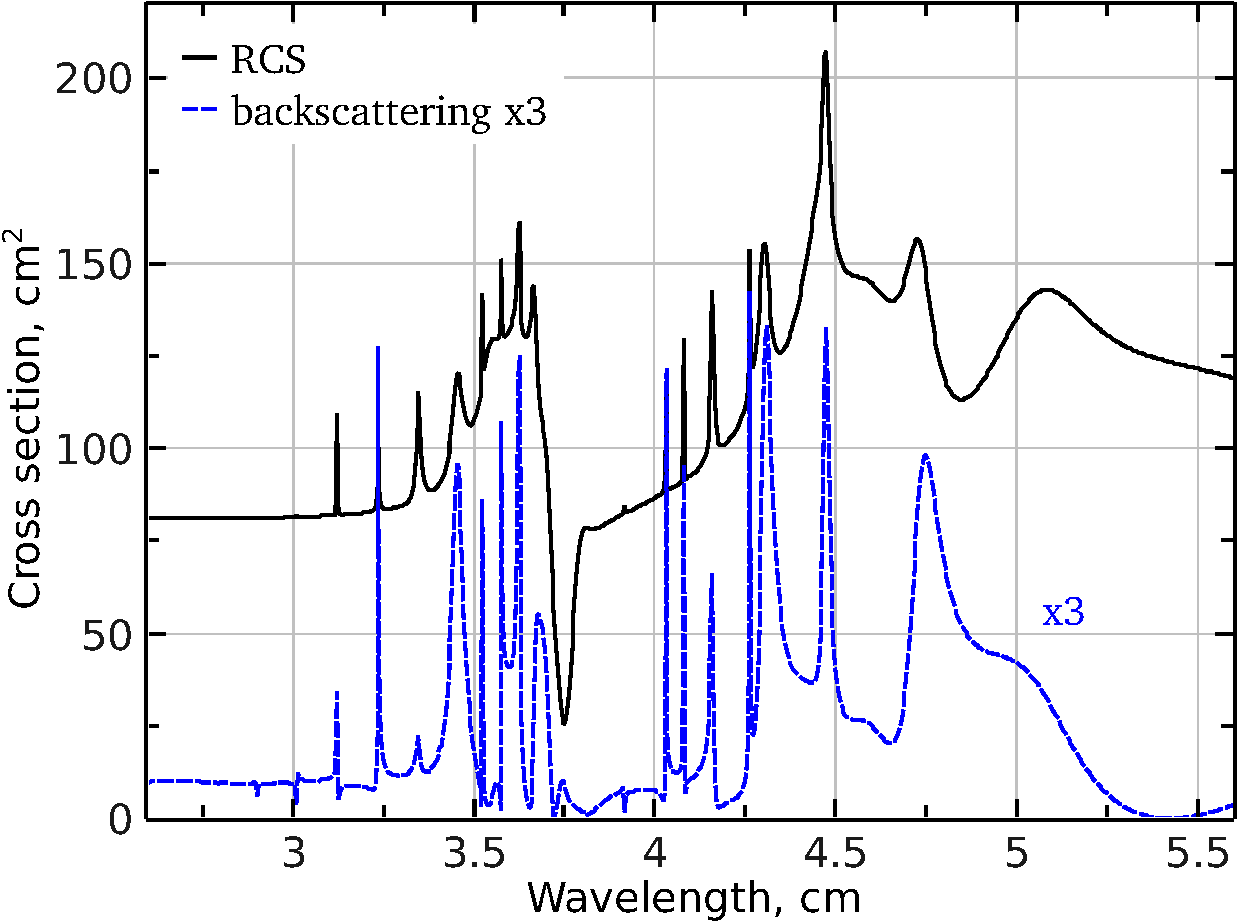
\includegraphics[width=0.47\textwidth]{w08-spectra}%
  \caption{Спектры TSCS и сечения обратного рассеяния, полученные в
    Scattnlay~\cite{Pena-scattnlay-2009} для двухдолинного дизайна,
    использованного при моделировании в пакете CST. Масштаб сечения
    для кривой обратного рассеяния увеличен в три раза.  Толщина
    покрытия $W=0.21\lambda$. Относительно непокрытой мишени $\Delta =-51.9$\%.     %TODO add    bare target spectra
    \label{fig:CST-design-spectra}}%
  % TODO Zero-backscattering can be disscused with Limonov and
  % Rybin. They can do additional review of the paper.
\end{figure}
% the CST rcs 25.4445 Mie 25.3412
Результаты компьютерного моделирования в пакете CST подтвердили
результаты расчётов с использованием теории Ми (25.44~см$^2$ и
25.34~см$^2$ соответственно).

Стационарное распределение поля (амплитуда  и фаза на
Рис.~\ref{fig:CST-Ex}) на частоте ${f = 8}$~ГГц были получены при
использовании алгоритмов CST в частотной области для разупорядоченной
тетрагональной сетки.
\begin{figure}
  \centering{
    % Use pdfcrop to remove white margins
    \begin{minipage}[h]{0.47\textwidth}
      a)\hfill
      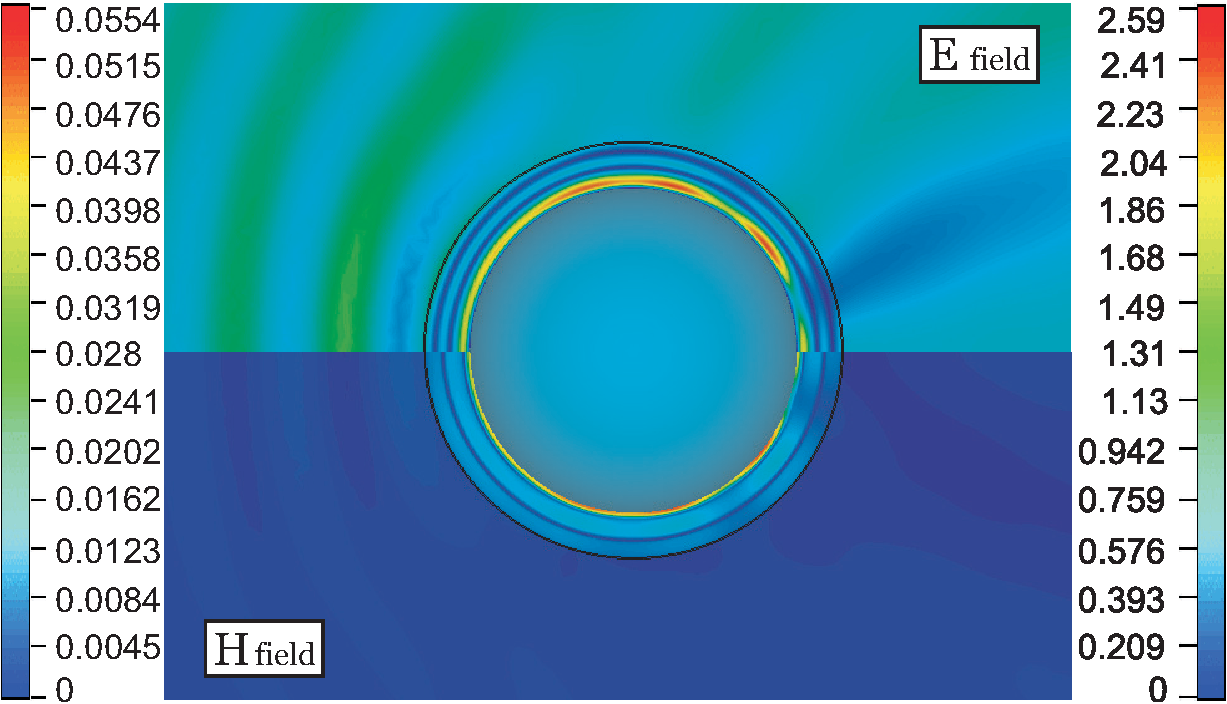
\includegraphics[width=0.95\textwidth]{W08-planeYZ-E-H-abs}%
    \end{minipage}\\%
    \begin{minipage}[h]{0.47\textwidth}
      b)\hfill
      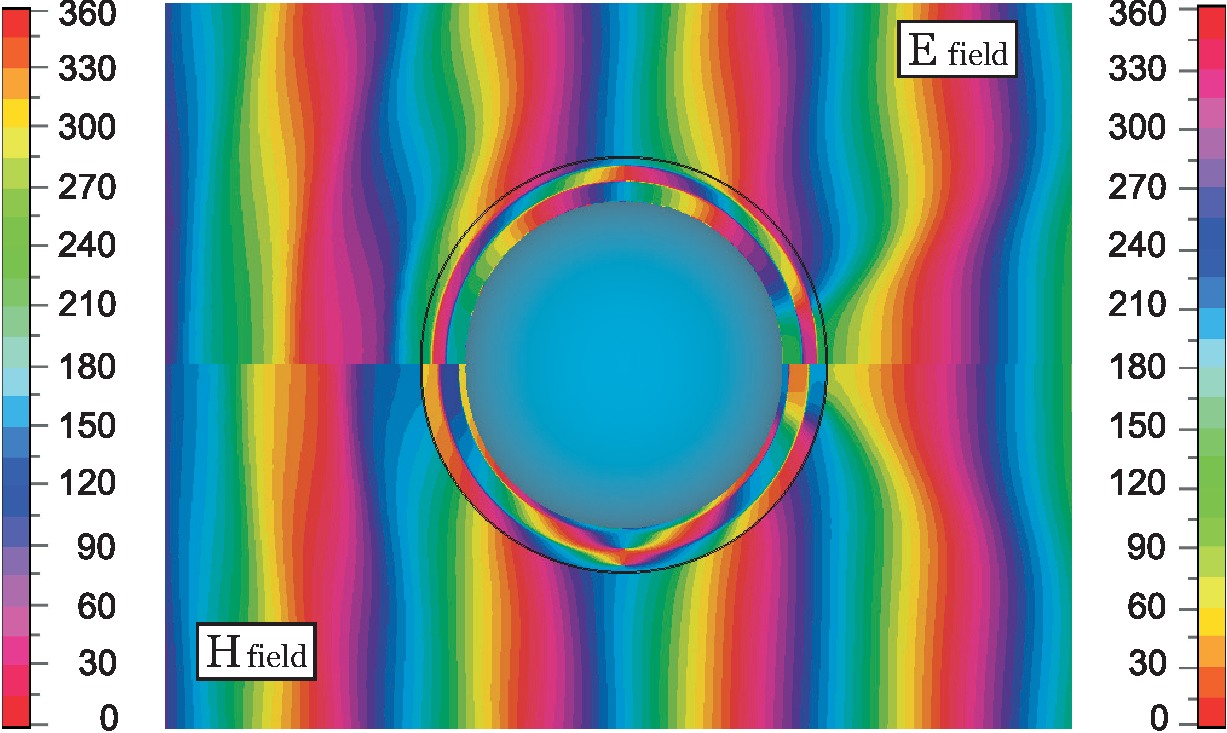
\includegraphics[width=0.95\textwidth]{W08-planeYZ-E-H-phase}%
    \end{minipage}%
      \caption{Амплитуда (a) и фаза (b) электрического (верхняя
        половина) и магнитного (нижняя половина) поля для
        двухдолинного дизайна. Окружности чёрного цвета обозначают
        границы внешнего слоя в покрытии.   Плоскость рисунка
        перпендикулярна плоскости поляризации электрического поля в
        падающей волне и проходит через центр мишени.  Амплитуда
        магнитного поля (левая шкала) измеряется в А/м, электрического
        поля (правая шкала) в В/м.  Фаза измеряется в градусах.
        \label{fig:CST-Ex}}%
  }
\end{figure}
Полное число ячеек в сетке составило около 4-х миллионов.  Для того
чтобы уменьшить моделируемый объём, мы использовали плоскости
симметрии.  Было выбрано открытое граничное условие с отражательной
способностью -40~dB.  Источник плоской волны расположен слева от
сферической мишени, плоскость поляризации электрического поля
перпендикулярна плоскости рисунка.

Необходимо отметить несколько особенностей распределения поля внутри
покрытия. 1) Электромагнитное поле в основном сконцентрировано во
внутренних слоях покрытия. 2) Присутствует нечто вроде антикорреляции
между минимумами и максимумами пространственного распределения
амплитуд электрического и магнитного полей: максимум электрического
поля соответствует минимуму магнитного и наоборот. 3) Существуют
тонкие <<переключающие>> слои с быстрым изменением фазы.  Прохождение
волны сквозь эти слои в радиальном направлении приводит к перевороту
её фазы на половину периода, далее идёт толстый слой перевёрнутой
фазы.  Положение <<переключающих>> слоёв совпадает с минимумами
амплитуды того поля, чья фаза переворачивается.

Давайте проследим за электрическим и магнитным полем, проходящим
через <<переключающие>> слои.  Такие слои можно эффективно
рассматривать как области резкого замедления распространения поля,
причиной которого является интерференция падающей и рассеянной волны.
Кроме того, плоскость постоянной фазы в области между
<<переключающими>> слоями имеет предпочтительное направление движения
в тангенциальном направлении.  Таким образом, один из возможных путей,
по которому может пойти падающая волна, выглядит следующим образом:
волна замедляется при прохождении сквозь <<переключающий>> слой, далее
она движется в радиальном направлении вдоль этого слоя,
замедляется ещё раз, проходя <<переключающий>> слой в обратном
направлении, и покидает покрытие.  Вследствие использованного дизайна
показателя преломления  набег фазы волны, проходящей внутри покрытия,
относительно волны, которая двигалась снаружи, оказывается в точности
равен полному периоду волны.  В результате поле, которое
распространялось подобным образом, не возмущает плоскость постоянной
фазы за мишенью.  Указанное поведение можно также трактовать с позиций
теории компенсации рассеяния~\cite{alu} со следующим дополнением.  В
нашем случае наличие антипараллельных векторов локальной
поляризуемости  вызвано наличием <<переключающих>> слоёв, приводящих к
изменению направления вектора электрического поля на противоположное.

В случае двухдолинного дизайна возникает два <<переключающих>> слоя.
Внешний слой работает указанным выше образом, внутренний слой работает
аналогично, но с небольшим отличием.  Набег фазы волны, проходящей
через внутренний слой, оказывается равен двум периодам.

Предложенное физическое описание механизма уменьшения полного сечения
рассеяния позволяет сделать простое предсказание.  При рассмотрении
указанных дизайнов во временной области установление стационарного
распределения амплитуды поля в области геометрической тени займёт
больше времени в случае двухдолинного дизайна по сравнению с
однодолинным.  

\section{Заключение}
Анализ этого и аналогичных графиков для других значений отношения
радиуса к длине волны~(рисунок~\ref{img:rcs-overview-r14-42}) позволил
выявить ряд характерных особенностей. Например, существует некое
пороговое значение толщины, после которого становится возможным
стабильное получение дизайнов, обеспечивающих заметное уменьшение
сечения рассеяния. При этом наилучшие показатели обеспечивают дизайны
характерной структуры, где несколько слоёв с высоким показателем
преломления окружают группу слоёв с низким показателем
преломления. Увеличение общей толщины покрытия приводит к переходу от
дизайнов в одной такой группой (рисунок~\ref{img:designs}(а)) к
дизайнам с двумя группами (рисунок~\ref{img:designs}(б)).




Адаптивный метод дифференциальной эволюции может быть успешно
использован для оптимизации полностью диэлектрических многослойных
покрытий в целях снижения рассеяния от сферических мишеней.  Были
найдены профили с оптимальным показателем преломления для различных
размеров мишени и толщин покрытия.  Были обнаружены одно- и
двухдолинные дизайны, которые оказались оптимальными для различных
геометрических параметров покрытия.  Для заданной максимальной
величины показателя преломления существует некая критическая толщина
покрытия, до который крайне тяжело найти дизайны покрытия с
маскирующим эффектом.  Для толщины покрытия больше критической
возникает переход от однодолинного дизайна к двухдолинному.  После
перехода существенного уменьшения TSCS не наблюдалось.  Мы
предполагаем, что также возможно существование многодолинных дизайнов,
однако мы не смогли их обнаружить по причине ограниченных
вычислительной мощности и времени.  Полученные дизайны дают
возможность для реализации маскировки без использования магнитных и
анизотропных метаматериалов.
   


TODO перестановки в пространстве для хаотического дизайна.

\underline{\textbf{Третья глава}} посвящена исследованию свойств
многослойных сферических маскирующих покрытий.

% ГОСТ Р 7.0.11—2011
% 5.3.9 На все иллюстрации должны быть приведены ссылки в тексте
% диссертации. При ссылке следует писать слово «Рисунок» с указанием
% его номера.

Сильной стороной теории Ми является возможность получать распределение
электрического и магнитного поля как внутри, так и вокруг изучаемой
наночастицы, вычислять значение фазы полей, а также строить линии
потока энергии.  Например, для структуры, изображённой на
рисунке~\ref{img:designs}(а), было рассчитано распределение фазы
электрического поля в окружающем частицу пространстве и внутри
покрытия (рисунок~\ref{img:field-phase}(а)).  Из рисунка видно, что
волна, проходящая через маскирующее покрытие, испытывает задержку фазы,
приблизительно равную $2\pi$. Другими словами, такой дизайн приводит к
тому, что электромагнитная волна после распространения внутри покрытия
на выходе оказывается в фазе с волной, которая двигалась в окружающем
пространстве.  Это, в свою очередь, подавляет картину интерференции в
дальнем поле и, в конечном итоге, объясняет возникающий маскирующий
эффект.

Иначе выглядит распределение фазы электрического поля на
рисунке~\ref{img:field-phase}(б), тут волна внутри покрытия на всей его
протяжённости движется в фазе с волной в окружающем пространстве. Это
стало возможным из-за использования в оптимизации материалов с
${\varepsilon<1}$, что соответствует маскировке объекта во вмещающей
среде, в которой скорость распространения света ниже, чем внутри
маскирующего покрытия.  Такие покрытия отличаются характерным дизайном
(рисунок~\ref{img:designs}(в)), в котором один слой с высоким
показателем преломления находится между слоями с ${\varepsilon<1}$.
\begin{figure}[t]
  \begin{minipage}[ht]{0.49\linewidth}
    \centering{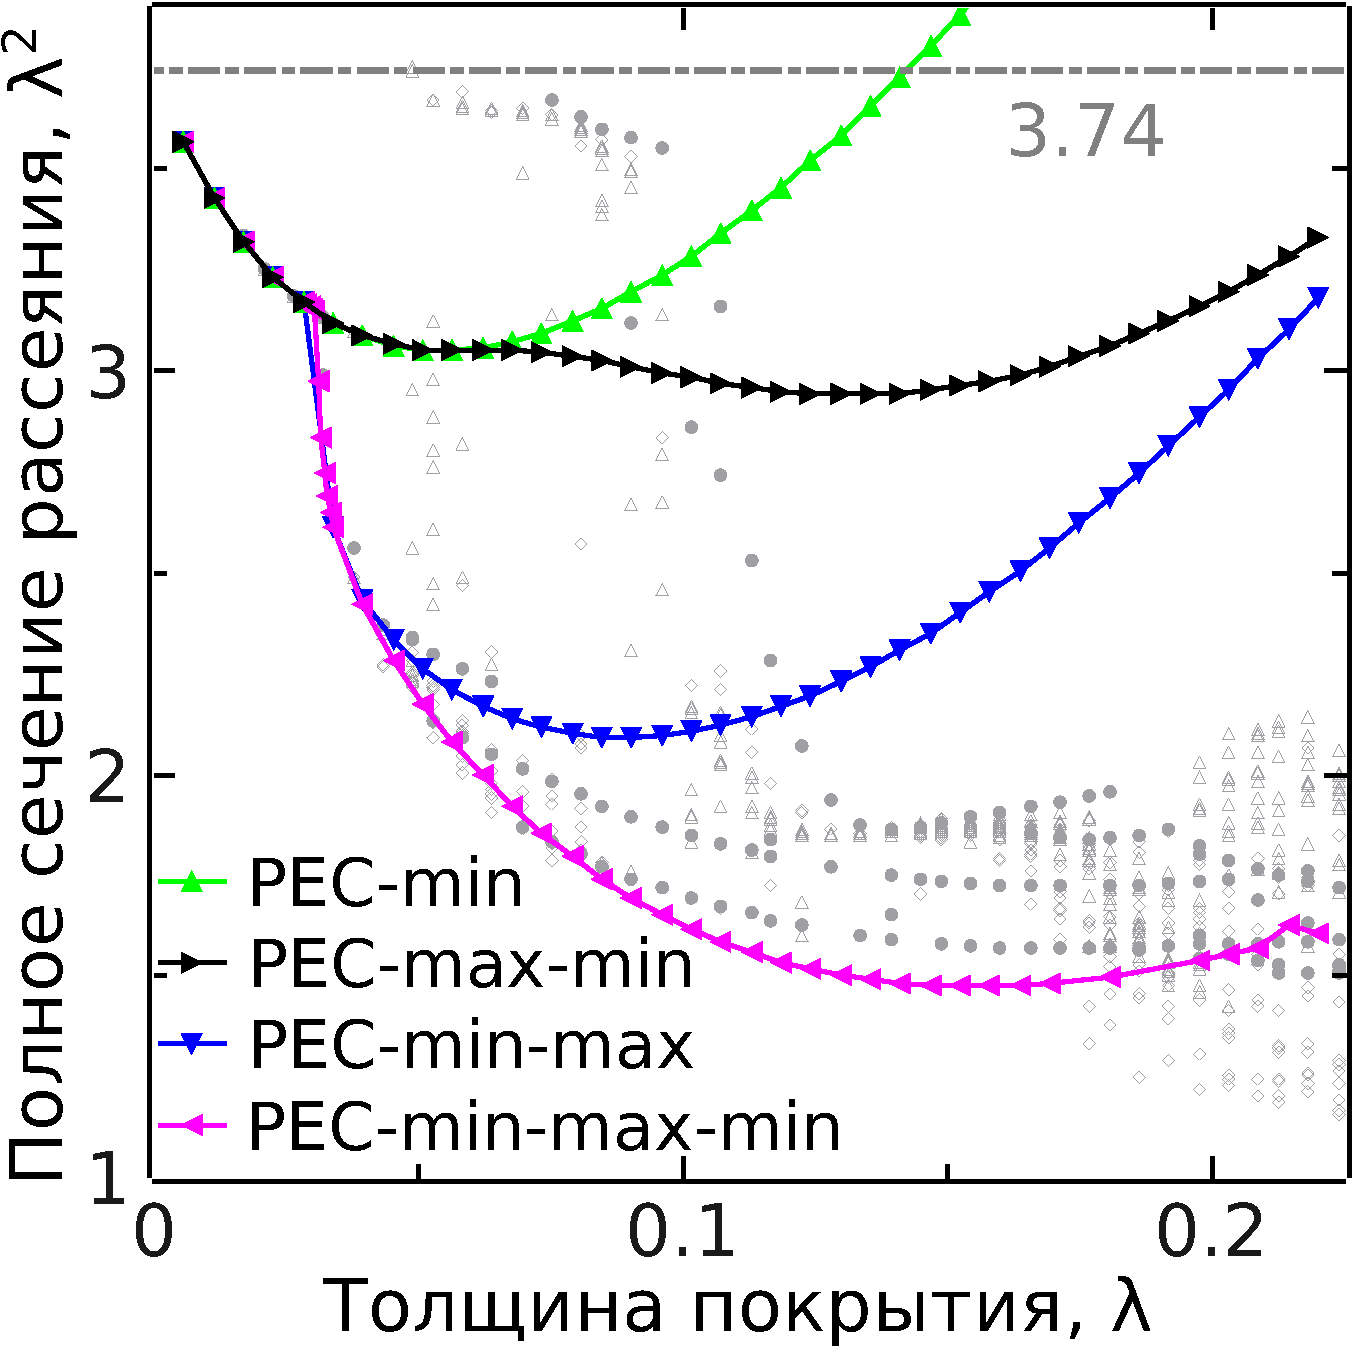
\includegraphics[width=0.95\linewidth]{rcs-overview-index07-DI} \\ а)}
  \end{minipage}
  \hfill
  \begin{minipage}[ht]{0.49\linewidth}
    \centering{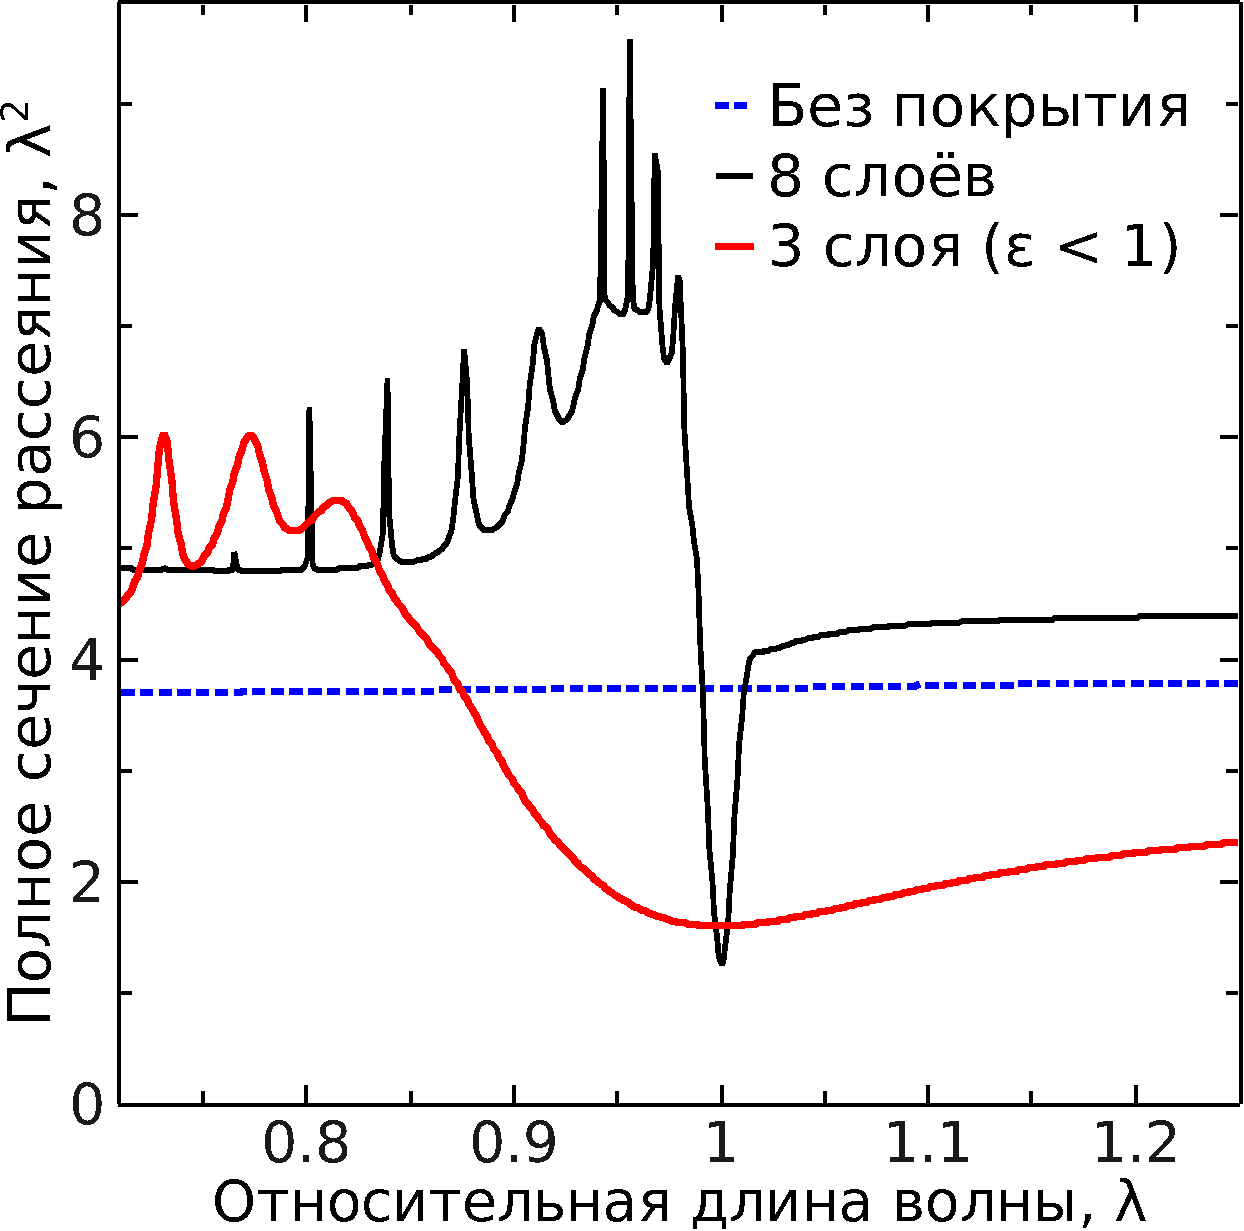
\includegraphics[width=0.95\linewidth]{index07-spectra} \\ б)}
  \end{minipage}
  \caption{а) Результат оптимизации покрытий с чередующимися слоями из
    большого $\varepsilon$ и ${\varepsilon<1}$. б) Спектры частицы
  без покрытия и с маскирующими покрытиями: из 8-ми слоёв диэлектрика и
  из 3-х слоёв с применением ${\varepsilon<1}$.}
  \label{img:min-max-min}  
\end{figure}

Обнаруженная закономерность позволила сформулировать гипотезу,
что для создания маскирующего покрытия достаточно использовать всего
два материала: с большим $\varepsilon$ и ${\varepsilon<1}$, а в
качестве параметров оптимизации можно использовать толщину каждого
слоя. Эта гипотеза была проверена численно, результаты оптимизации
отображены на рисунке~\ref{img:min-max-min}(а). Оказалось, что для
большей части рассматриваемого диапазона общей толщины покрытия 
достаточно всего трёх слоёв, чтобы получить приблизительно то же
уменьшение полного сечения рассеяния, что и в случае применения 4, 8 и
16 слоёв равной толщины, когда при оптимизации
изменялись материальные параметры каждого слоя.

Особый интерес представляет различие в спектрах рассеяния для случаев
наличия и отсутствия материала с ${\varepsilon<1}$ в оптимизированном
покрытии.  При расчёте спектров для рисунка~\ref{img:min-max-min}(б) не
учитывалось наличие в материалах дисперсии и сопутствующих потерь,
поэтому их форма полностью определяется дизайном маскирующего
покрытия. Хорошо виден относительно узкий резонанс, который определяет
маскирующие свойства покрытия на основе диэлектриков. Использование
материала с ${\varepsilon<1}$ позволило в несколько раз расширить
диапазон длин волн, где наблюдается подавление рассеяния. 

\clearpage